\documentclass[10pt,psamsfonts]{amsart}

%-------Packages---------
\usepackage{amssymb,amsfonts}
%\usepackage[all,arc]{xy}
\usepackage{enumerate}
%\usepackage{mathrsfs}
\usepackage{subcaption}
\usepackage{graphicx}
\usepackage{caption}
\usepackage[margin=0.3in]{geometry}

%--------Theorem Environments--------
%theoremstyle{plain} --- default
\newtheorem{thm}{Theorem}[section]
\newtheorem{cor}[thm]{Corollary}
\newtheorem{prop}[thm]{Proposition}
\newtheorem{lem}[thm]{Lemma}
\newtheorem{conj}[thm]{Conjecture}
\newtheorem{quest}[thm]{Question}

\theoremstyle{definition}
\newtheorem{defn}[thm]{Definition}
\newtheorem{defns}[thm]{Definitions}
\newtheorem{con}[thm]{Construction}
\newtheorem{exmp}[thm]{Example}
\newtheorem{exmps}[thm]{Examples}
\newtheorem{notn}[thm]{Notation}
\newtheorem{notns}[thm]{Notations}
\newtheorem{addm}[thm]{Addendum}
\newtheorem{exer}[thm]{Exercise}

\theoremstyle{remark}
\newtheorem{rem}[thm]{Remark}
\newtheorem{rems}[thm]{Remarks}
\newtheorem{warn}[thm]{Warning}
\newtheorem{sch}[thm]{Scholium}

\makeatletter
\let\c@equation\c@thm
\makeatother
\numberwithin{equation}{section}

\bibliographystyle{plain}

%--------Meta Data: Fill in your info------
%\title{Homework 1}

%\author{Won I. Lee}

%\date{July 30, 2016}


\begin{document}
	
%\maketitle

\begin{center}
	{\bf Homework 1}
\end{center}

\section{Implement Gradient Descent}

In this section, we investigate the performance of gradient descent-based algorithms for minimizing scalar functions of vector arguments. In particular, we consider the following functions: 1) the negative Gaussian function:
$$f(x) = -\frac{1}{\sqrt{(2\pi)^n |\Sigma|}} \exp\left[ -\frac{1}{2}(x-u)^T\Sigma^{-1}(x-u) \right]$$
and 2) the quadratic bowl function $f(x) = \frac{1}{2}x^TAx - x^Tb$.
\subsection{Initialization and Hyperparameters} We first explore the batch gradient descent algorithm. For loss function $f(x)$, the gradient descent algorithm performs $x = x - \eta \nabla f(x)$
where $\eta$ is the step size. These iterations continue until a convergence threshold is met, i.e. $|f(x) - f(\tilde{x})| < \epsilon$, where $x, \tilde{x}$ are successive iterations. We investigate the dependence of this algorithm on the initialization of the algorithm as well as its hyperparameters, namely the step size $\eta$ and the convergence threshold $\epsilon$. Throughout the experiments, we fix the following parameters of the functions $u = (10, 10),\Sigma = \begin{pmatrix} 1000 & 0 \\ 0 & 1000\end{pmatrix}$ and $A = \begin{pmatrix} 10 & 5 \\ 5 & 10\end{pmatrix},b = (400, 400)$.

First, we note that the large variance in the negative Gaussian density yields small objective function values (scaled by the reciprocal of the determinant of $\Sigma$), as well as small gradients. Thus, we consider only large step sizes that will yield noticeable increments in the values of $x$; otherwise, no learning is achieved. Similarly, we only consider very small $\epsilon$ for the same reasons.

The results are shown in {\bf Figure 1} for the negative Gaussian function, where the $z$-axis is the squared distance. We have used step sizes of $10^5, 10^6, \dots, 10^10$ and convergence criteria of $10^{-10}, 10^{-11}, \dots, 10^{-20}$. The plots reveal two major points. First, for any choice of initialization and step size used in the experiments, gradient descent does not converge to a suitable solution until $\epsilon$, the convergence threshold, is sufficient small. As the plots demonstrate, we require $\epsilon \approx 10^{-15}$ or $\log(\epsilon) \approx -35$ before the squared error falls to negligible values. Second, the step size must bee sufficiently large before convergence is achieved, in the same vein as the convergence threshold. Even for suitable $\epsilon$ values, a relatively small step size (i.e. $10^5$) does not yield approximate convergence to the correct solution. Indeed, for most cases, we require a step size of $\eta \approx 10^7$ before the suared loss becomes negligible. As discussed above, these issues are germane to the negative Gaussian function, due to the large determinant value effectively annihilating the step sizes unless sufficiently large.

On the other hand, the quadratic bowl function does not have such issues, and using large step sizes generally yields divergence. Indeed, even using $\eta = 1$ leads to diverging estimates for $\epsilon \approx 10^{-15}$. Thus, for this case we consider step sizes of $10^{-1}, 10^{-2}, \dots, 10^{-5}$ and similarly convergence criteria of $10^{-10}, 10^{-11}, \dots, 10^{-20}$. Results as shown in {\bf Figure 2} demonstrate a very similar behavior for the quadratic bowl function; the convergence threshold $\epsilon$ must be suitably small for convergence to the correct values. In this case, however, if the step size $\eta$ is too small, then no $\epsilon$ used in our experiments can yield convergence, unlike the case of the negative Gaussian, in which a suitably small $\epsilon$ would yield convergence in all step sizes. We must have a large enough step size (in this case $\eta \approx 0.01$) for convergence in this example.

\begin{figure}[b]
	\centering
	\begin{subfigure}[b]{0.23\textwidth}
	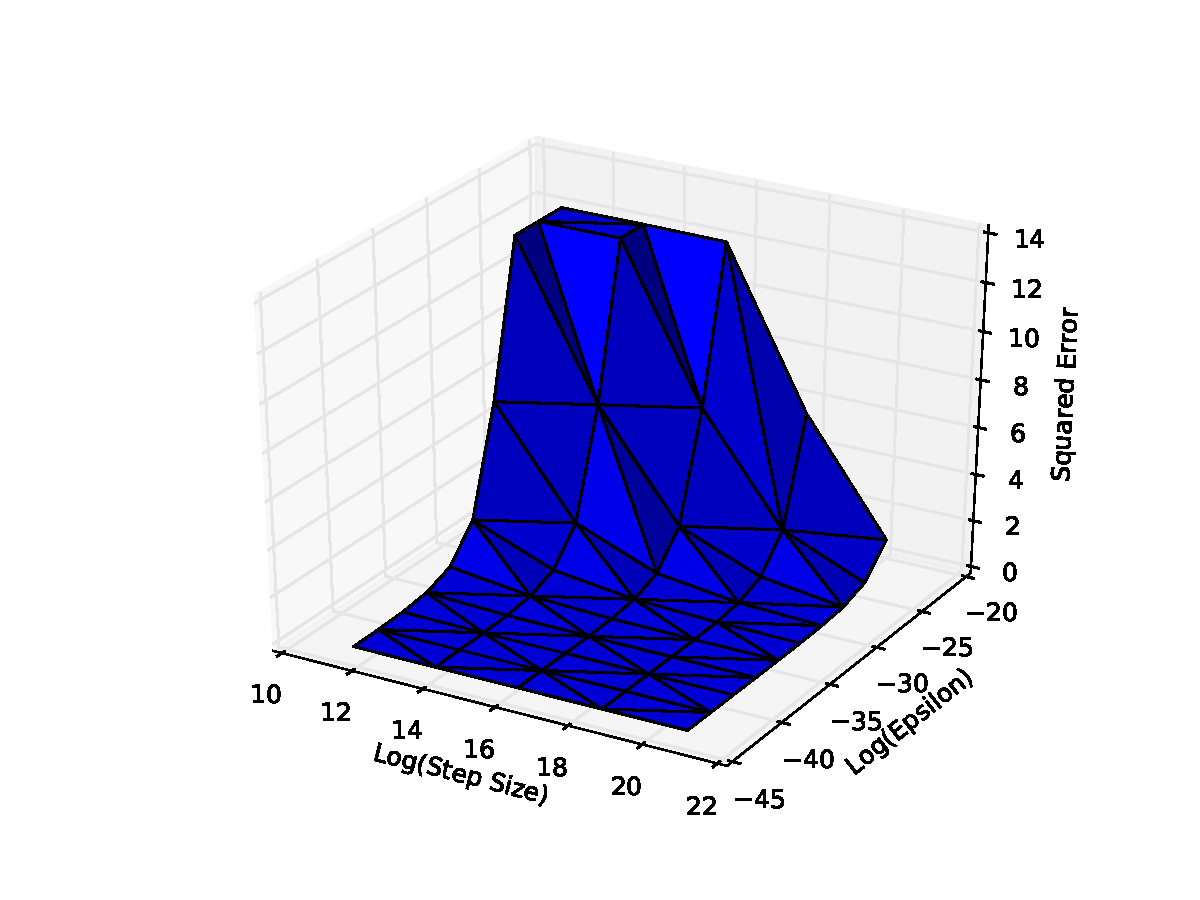
\includegraphics[width=\textwidth]{hw1_1-1_0.pdf}
	\caption{(1,1)}
	\end{subfigure}
\begin{subfigure}[b]{0.23\textwidth}
	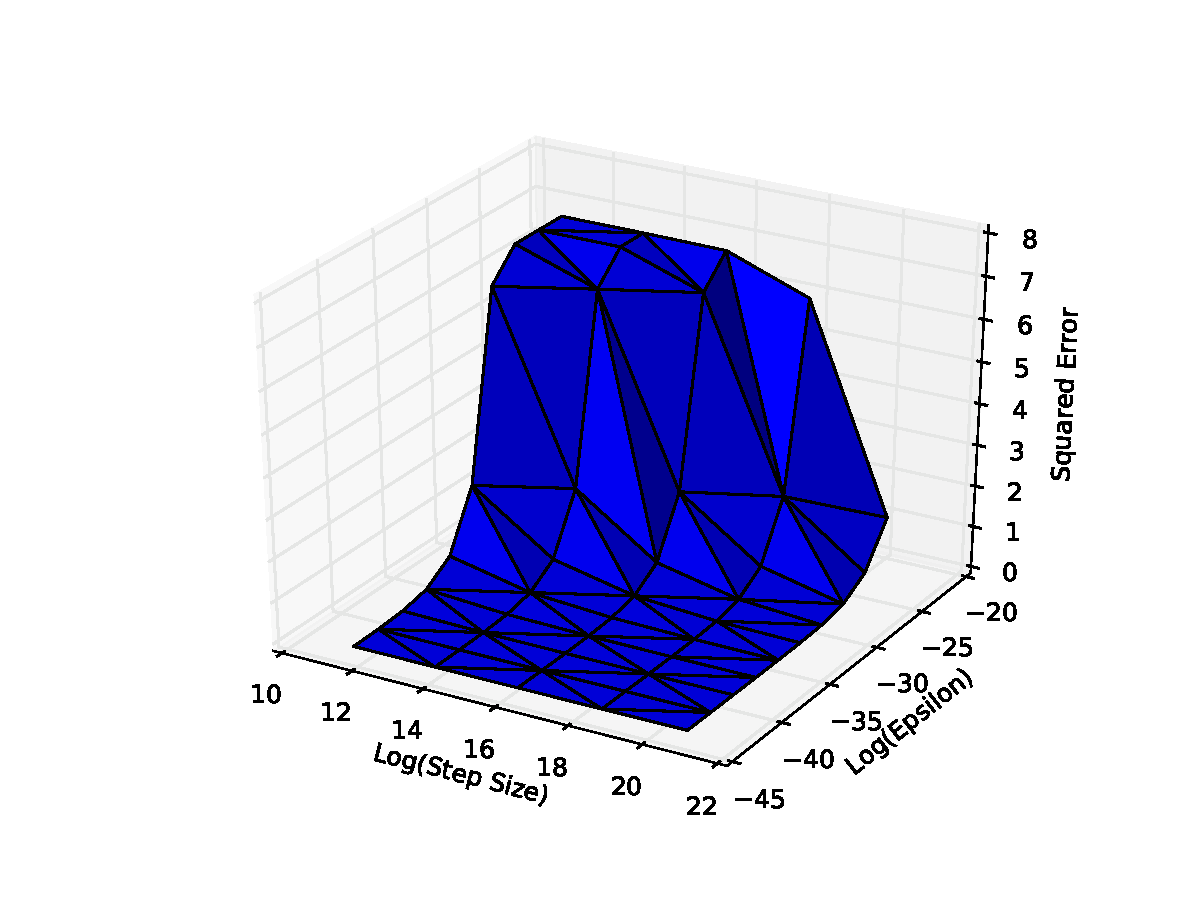
\includegraphics[width=\textwidth]{hw1_1-1_1.pdf}
	\caption{(5,5)}
\end{subfigure}
\begin{subfigure}[b]{0.23\textwidth}
	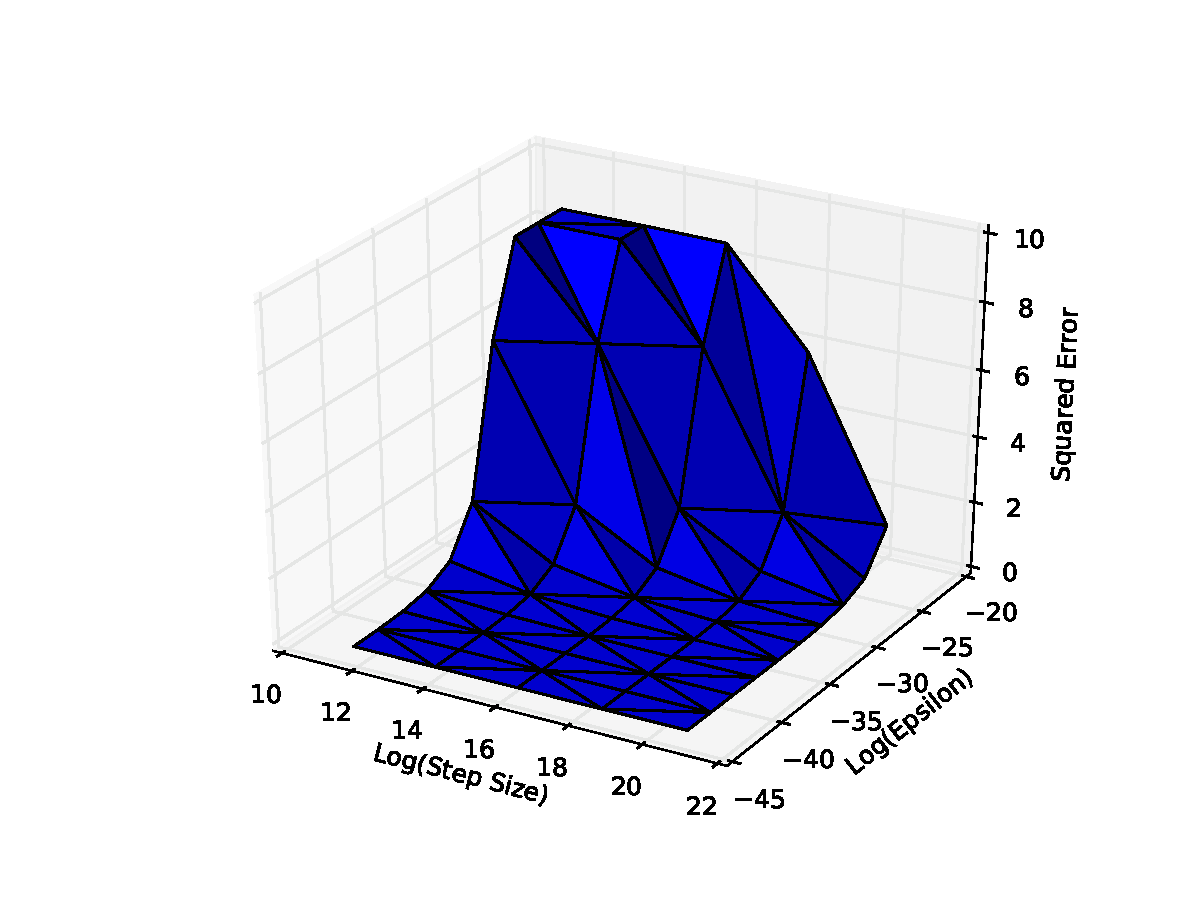
\includegraphics[width=\textwidth]{hw1_1-1_2.pdf}
	\caption{(1,9)}
	\end{subfigure}
	\begin{subfigure}[b]{0.23\textwidth}
		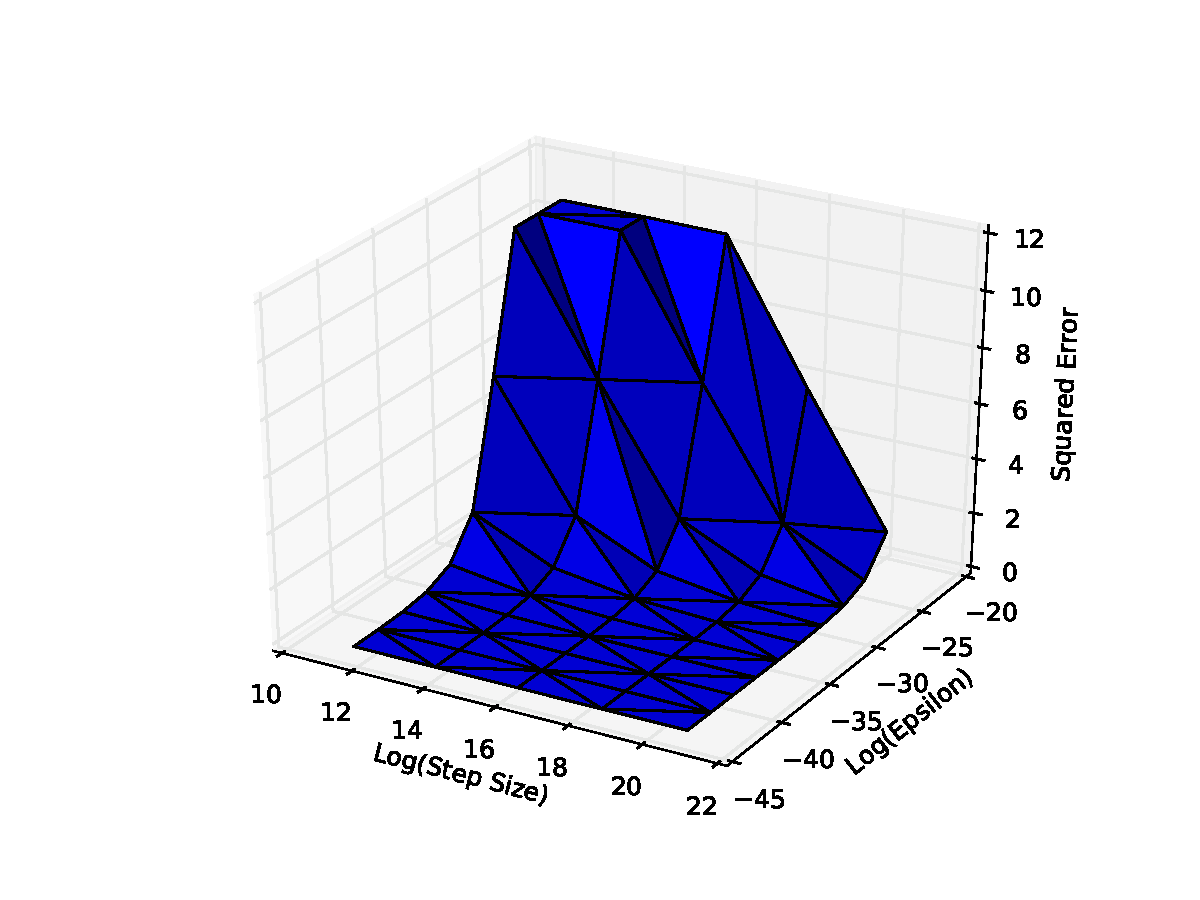
\includegraphics[width=\textwidth]{hw1_1-1_3.pdf}
		\caption{(20,15)}
		\end{subfigure}
\caption{Squared distance to correct solution $u$ using the negative Gaussian function for various starting points, step sizes, and convergence criteria. The labels on the plots are the starting points.}
\end{figure}

\begin{figure}
	\centering
	\begin{subfigure}[b]{0.23\textwidth}
		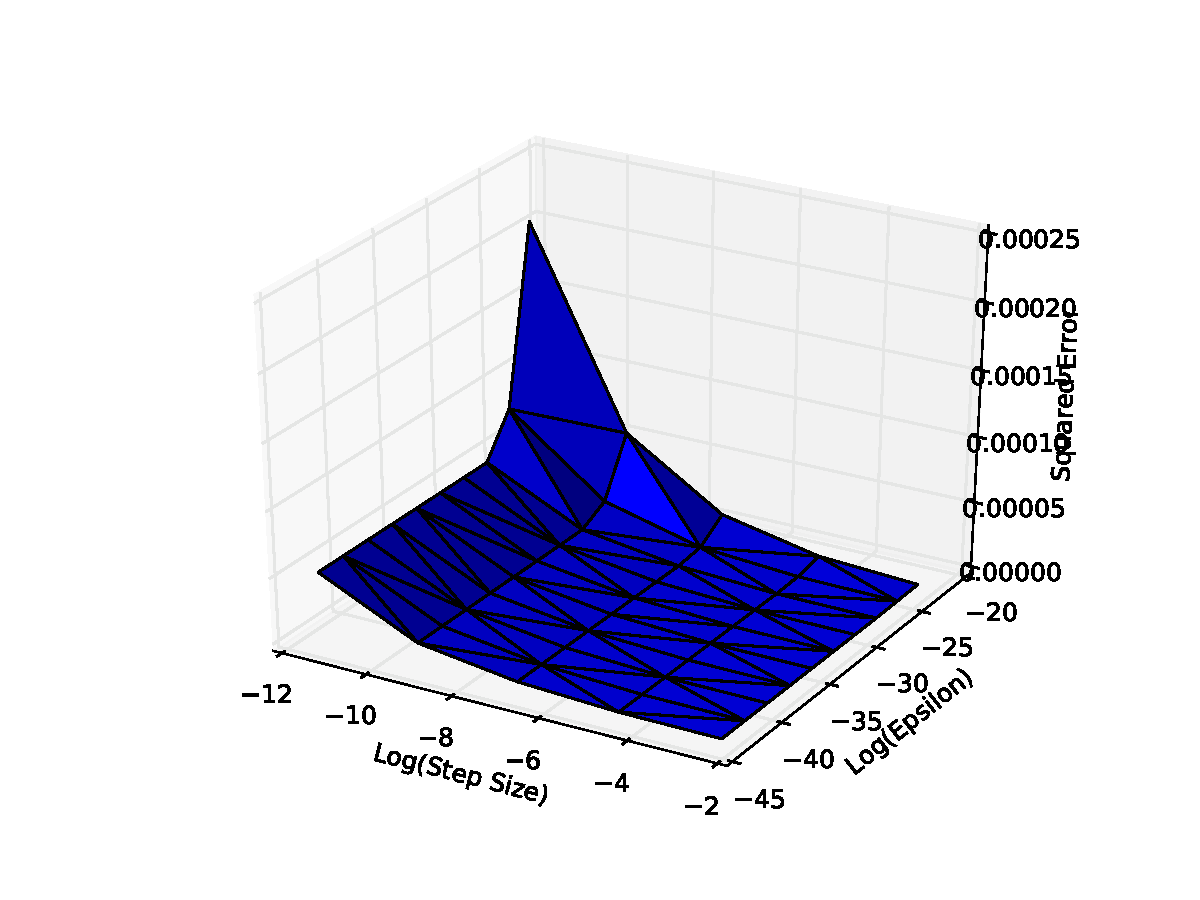
\includegraphics[width=\textwidth]{hw1_1-2_0.pdf}
		\caption{(1,1)}
	\end{subfigure}
	\begin{subfigure}[b]{0.23\textwidth}
		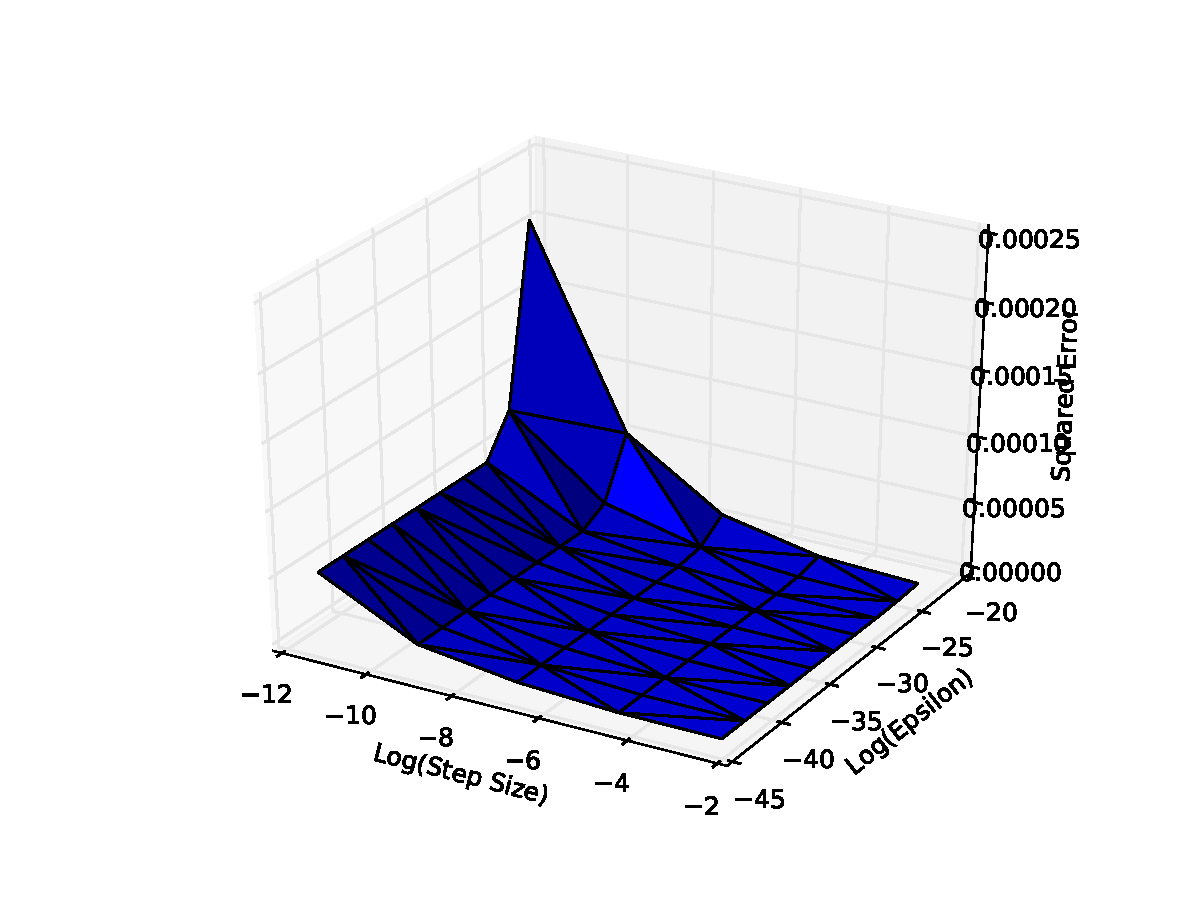
\includegraphics[width=\textwidth]{hw1_1-2_1.pdf}
		\caption{(5,5)}
	\end{subfigure}
	\begin{subfigure}[b]{0.23\textwidth}
		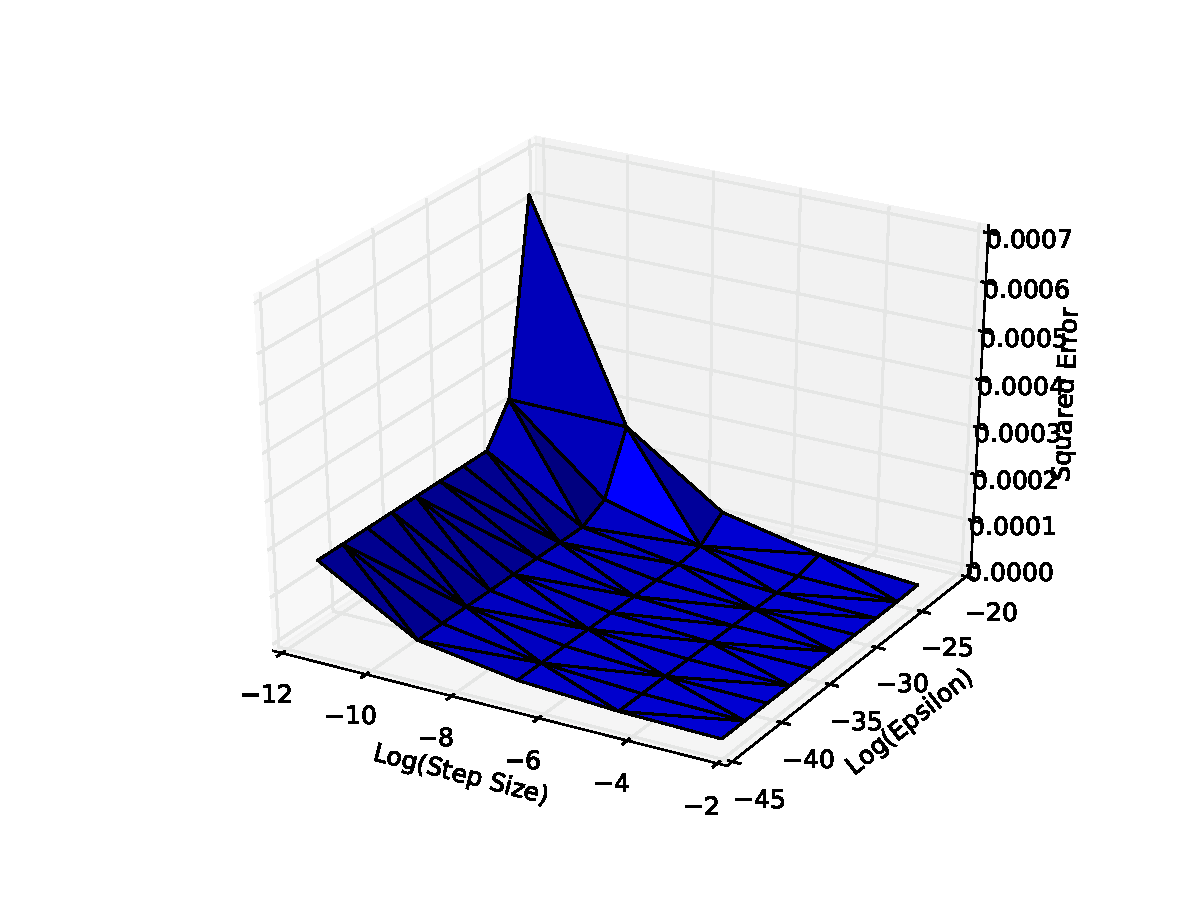
\includegraphics[width=\textwidth]{hw1_1-2_2.pdf}
		\caption{(1,9)}
	\end{subfigure}
	\begin{subfigure}[b]{0.23\textwidth}
		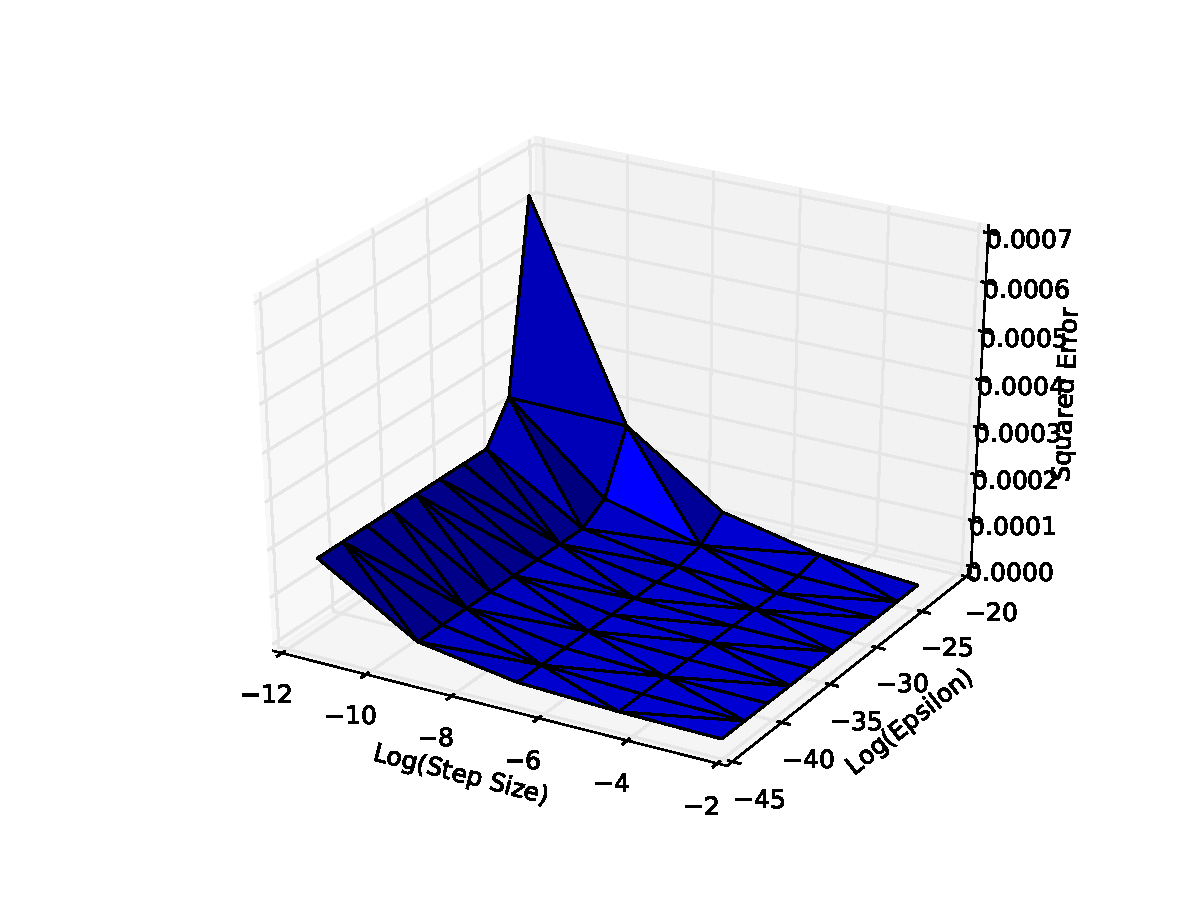
\includegraphics[width=\textwidth]{hw1_1-2_3.pdf}
		\caption{(20,15)}
	\end{subfigure}
	\caption{Squared distance to correct solution $u$ using the quadratic bowl function for various starting points, step sizes, and convergence criteria. The labels on the plots are the starting points.}
\end{figure}
	

\subsection{Comparison to Finite Differences} We compare the exact gradients obtained to finite difference approximations of the gradient using a central difference method:

$$\frac{\partial f(x)}{\partial x_i} \approx \frac{f(x + \delta e_i) - f(x - \delta e_i)}{2\delta}$$

where $\delta$ is the difference size and $e_i$ is a unit vector in the $i^{th}$ coordinate. We consider a number of different $\delta$ and compare the squared error between the true gradient and the finite approximation to the gradient. Namely, we compute the finite difference for $\delta = 1, 0.1, \dots, 10^{-4}$ and consider the points given in Figures 1 and 2. The result is given in {\bf Figure 3}, where we see that even for a step size of $\delta = 1$, we obtain a squared error of approximately $10^{-13}$ for the negative Gaussian and 0 for the quadratic bowl function (since it has a linear derivative). The nonzero squared error for smaller difference sizes for the quadratic bowl function is postulated to be due to numerical error, but even these are negligible. This demonstrates that for simple functions such as the two considered here, the finite difference gradient can be a cheap yet accurate approximation to the actual gradient.

\begin{figure}
\begin{subfigure}[b]{0.3\textwidth}
	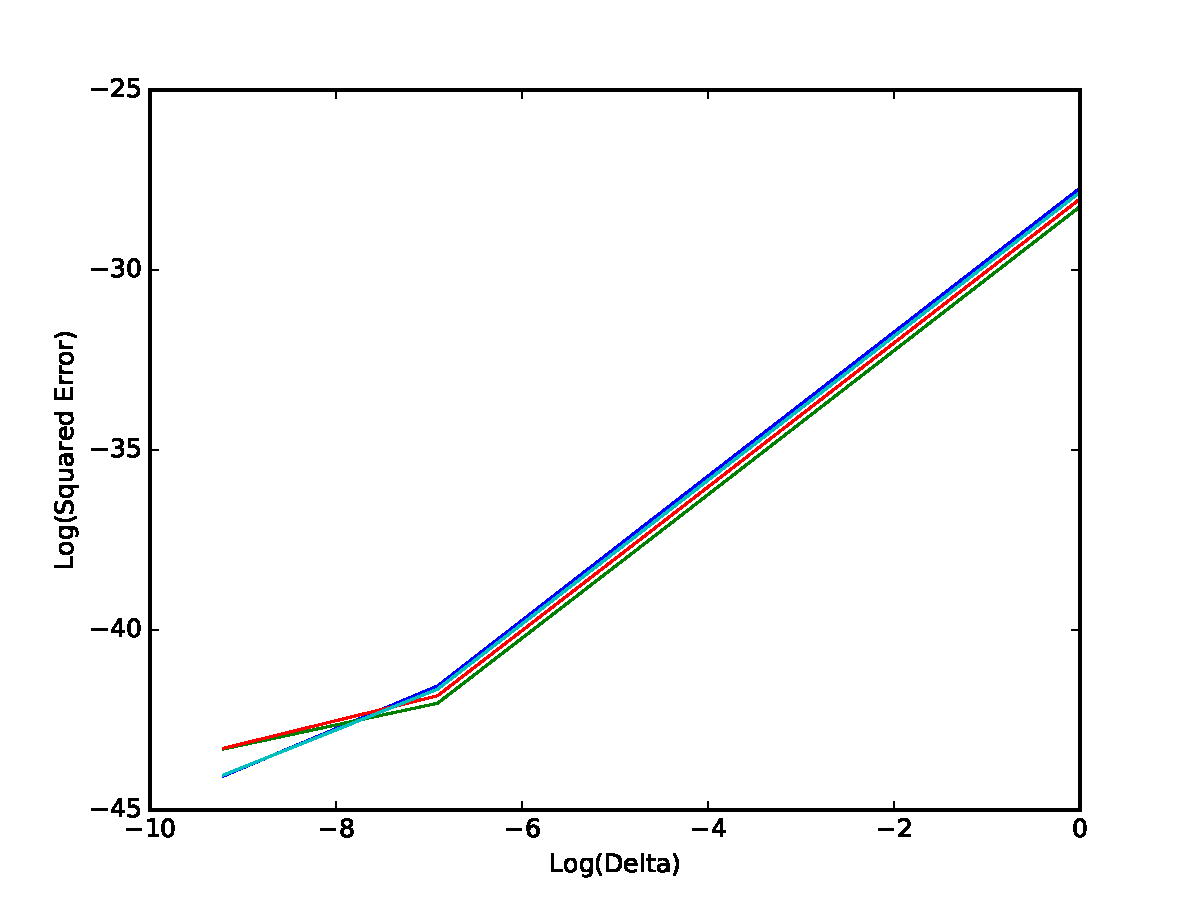
\includegraphics[width=\textwidth]{hw1_1-2a.pdf}
	\caption{Negative Gaussian}
\end{subfigure}
\begin{subfigure}[b]{0.3\textwidth}
	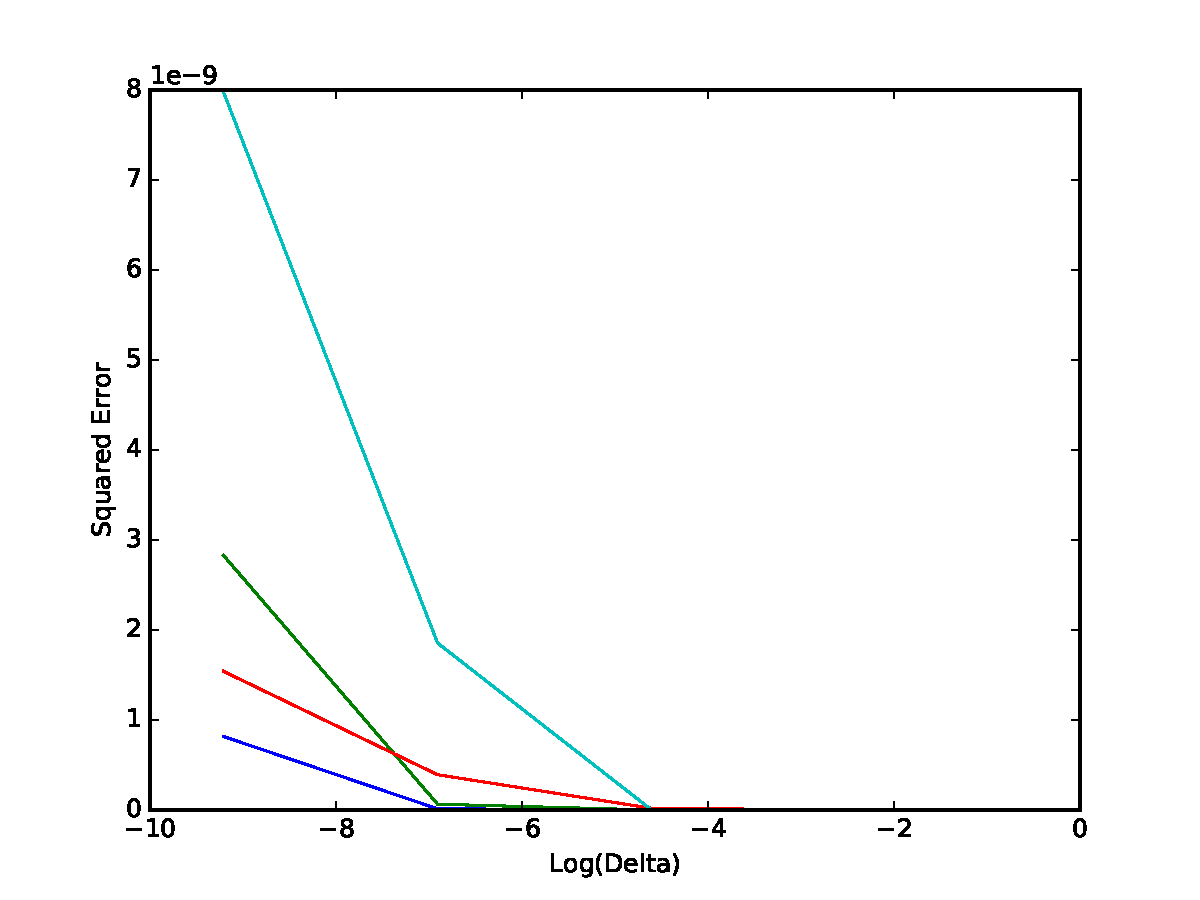
\includegraphics[width=\textwidth]{hw1_1-2b.pdf}
	\caption{Quadratic bowl}
\end{subfigure}
\caption{Squared error of finite difference gradient approximations compared to the exact gradients for differing step sizes.}
\end{figure}

\subsection{Batch vs. Stochastic Gradient Descent on Least Squares}

We now turn to the question of fitting parameter values for a linear model:
$$y = x^T\theta$$
and we want to estimate $\theta$, using a squared loss:
$$J(\theta) = \|X\theta - y\|^2$$
where $X$ is our model matrix. Our goal is to study the relative performance of batch and stochastic gradient descent on this problem. In order to do so, we first derive the batch gradient to be:
$$\nabla_{\theta} J(\theta) = 2X^T(X\theta - y)$$

In the stochastic gradient case, we have the following point-wise gradient:

$$\nabla_{\theta} J_i(\theta; x^{(i)}, y^{(i)}) = 2(x^{(i)T}\theta - y^{(i)}) x^{(i)}$$

We would like to understand how the two algorithms behave under similar conditions. Thus, we explore the accuracy (in terms of $L_2$ distance from the exact solution). That is, each iteration of the batch gradient descent counts as $n$ evaluations, where $n$ is the number of data points. Unfortunately, we found through empirical experiments that SGD simply does not converge to accurate values under typical Robbins-Monro annealing, i.e. $\eta_t = \eta/(\tau_0 + t)^{\kappa}$.
In fact, even when we chose initial $\theta_0$ to be the actual exact solution rounded to the nearest integer, SGD did not yield a reasonable solution. In all of these cases, SGD tended to converge prematurely, even with $\tau_0 = 0$ and $\kappa = 0.5$, the minimum value for the conditions to hold.

Thus, we consider values of $\tau_0, \kappa$ that may lie outside of the guarantees of the Robbins-Monro conditions. Moreover, having SGD use step size annealing while batch GD employs constant step sizes is not an apples-to-apples comparison; consequently, we employ the same step size annealing procedure in both algorithms, augmenting batch GD with such a procedure. We found that a starting step size of $\eta = 10^{-5}$ and convergence threshold of $\epsilon = 10^{-15}$ worked well for most experiments, as shown in the case of the negative Gaussian and quadratic bowl, and keep these fixed. On the other hand, we vary values of $\tau_0, \kappa$ and see how the accuracy and evaluation numbers of the two algorithms compare in these different situations. We also fix the initialization at $\theta_0 = (1, \dots, 1)$ for all experiments.

The results are shown in {\bf Figure 4}. We see that for the same value of $\tau, \kappa$, batch gradient descent uniformly dominates SGD in terms of squared error. Moreover, $\tau$, perhaps as expected, has little effect on the convergence of the algorithms, while $\kappa$ plays a significant role, especially for SGD. When $\kappa$ is too large, SGD terminates prematurely, as shown by part (C), where the number of evaluations of SGD for $\kappa > 10^{-4}$ is negligible compared to the lowest $\kappa$ case. This is directly tied to the accuracy of the SGD algorithm; in all but the smallest values of $\kappa$, the algorithm converges to a substantially inaccurate value. Thus, we see that it is critical to make sure that the annealing of the step sizes is sufficiently slow for the algorithm to converge to the correct value. However, having annealing that is too slow yields an exponential increase in number of evaluations, with negligible gains in squared error (i.e. $\kappa < 10^{-5}$).

\begin{figure}
		\begin{subfigure}[b]{0.3\textwidth}
			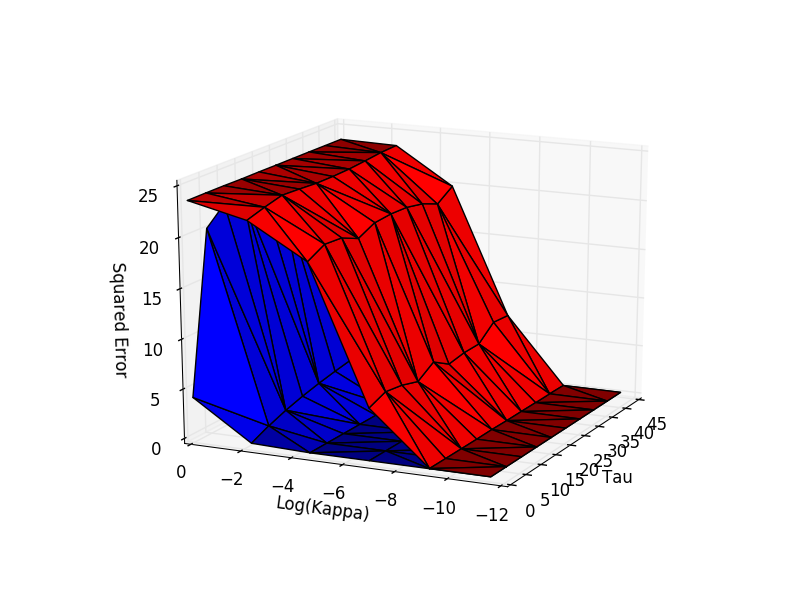
\includegraphics[width=\textwidth]{hw1_1-3_acc_both.png}
			\caption{Squared error for batch (blue) and stochastic (red) gradient descent.}
		\end{subfigure}
			\begin{subfigure}[b]{0.3\textwidth}
				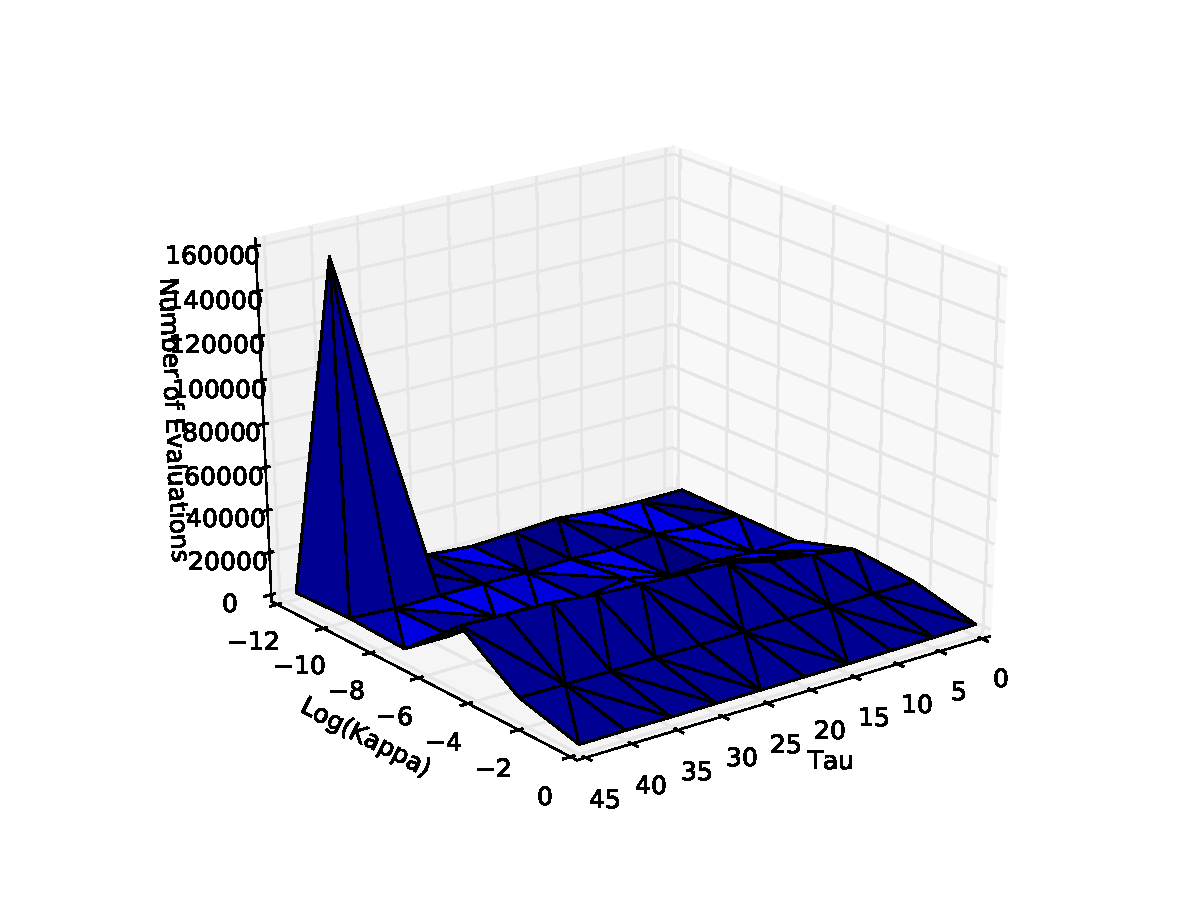
\includegraphics[width=\textwidth]{hw1_1-3_timeGD.pdf}
				\caption{Batch}
			\end{subfigure}
		\begin{subfigure}[b]{0.3\textwidth}
			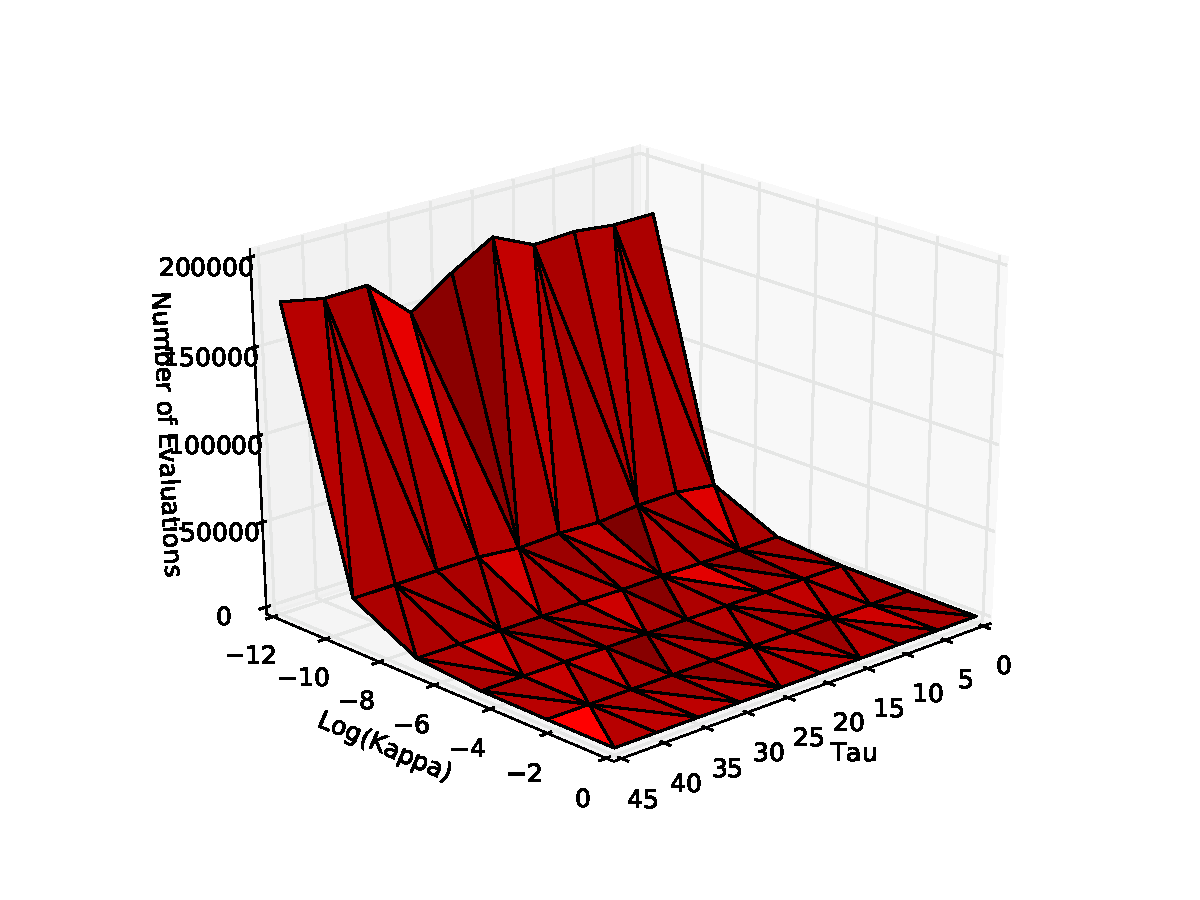
\includegraphics[width=\textwidth]{hw1_1-3_timeSGD.pdf}
			\caption{Stochastic}
		\end{subfigure}			
	\caption{(A) shows the squared error for the two algorithms, while (B) and (C) show number of gradient evaluations for batch and stochastic gradient descent, respectively.}
\end{figure}

\section{Linear Basis Function Regression}

We now turn to the question of linear regression using nonlinear basis functions. We consider the true data model:

$$y(x) = \cos(\pi x) + 1.5 \cos(2\pi x) + \epsilon$$
where $\epsilon$ is small random noise.

\subsection{Polynomial Basis} We start by exploring the suitability of polynomial basis functions for this model, varying the maximum degree of the polynomial terms; namely, we consider the basis:

$$\phi_0(x) = 1, \phi_1(x) = x, \dots, \phi_M(x) = x^M$$

We find, as expected, that lower-order polynomials (i.e. $M = 0, 1$) fail to fit the data well due to their simplicity, whereas polynomials of too high order (i.e. $M = 10$) overfit the data substantially. This is demonstrated in {\bf Figure 5}.

\begin{figure}
	\centering
	\begin{subfigure}[b]{0.24\textwidth}
		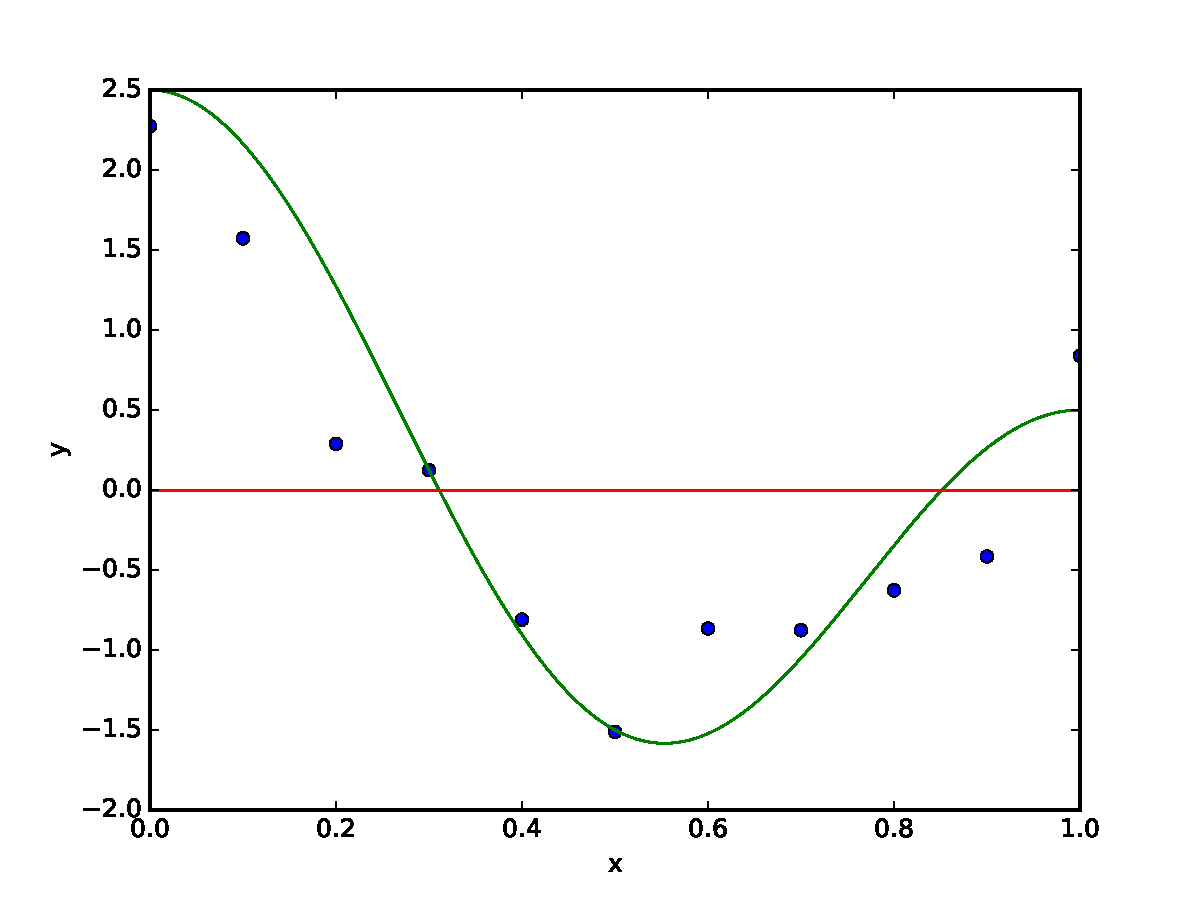
\includegraphics[width=\textwidth]{hw1_2-1_0.pdf}
		\caption{$M=0$}
	\end{subfigure}
	\begin{subfigure}[b]{0.24\textwidth}
		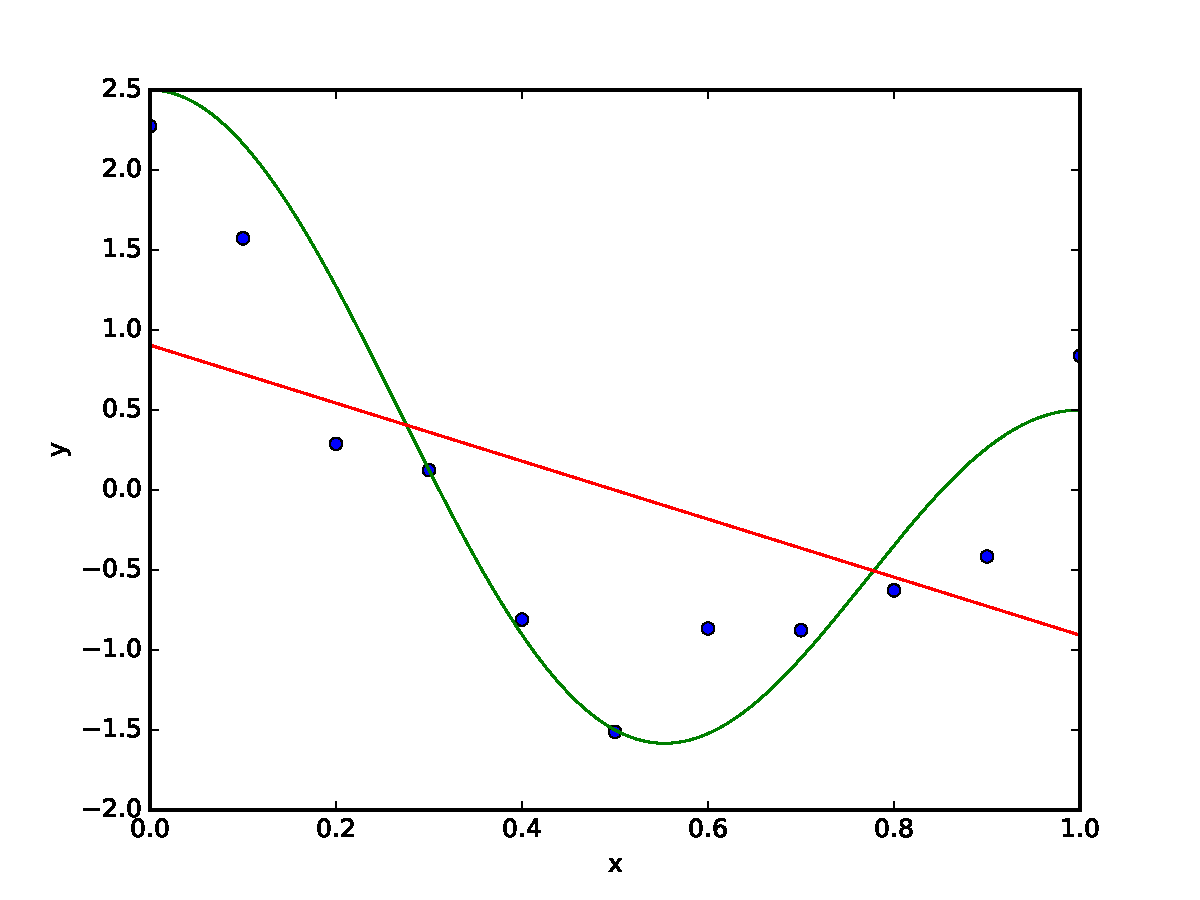
\includegraphics[width=\textwidth]{hw1_2-1_1.pdf}
		\caption{$M=1$}
	\end{subfigure}
	\begin{subfigure}[b]{0.24\textwidth}
		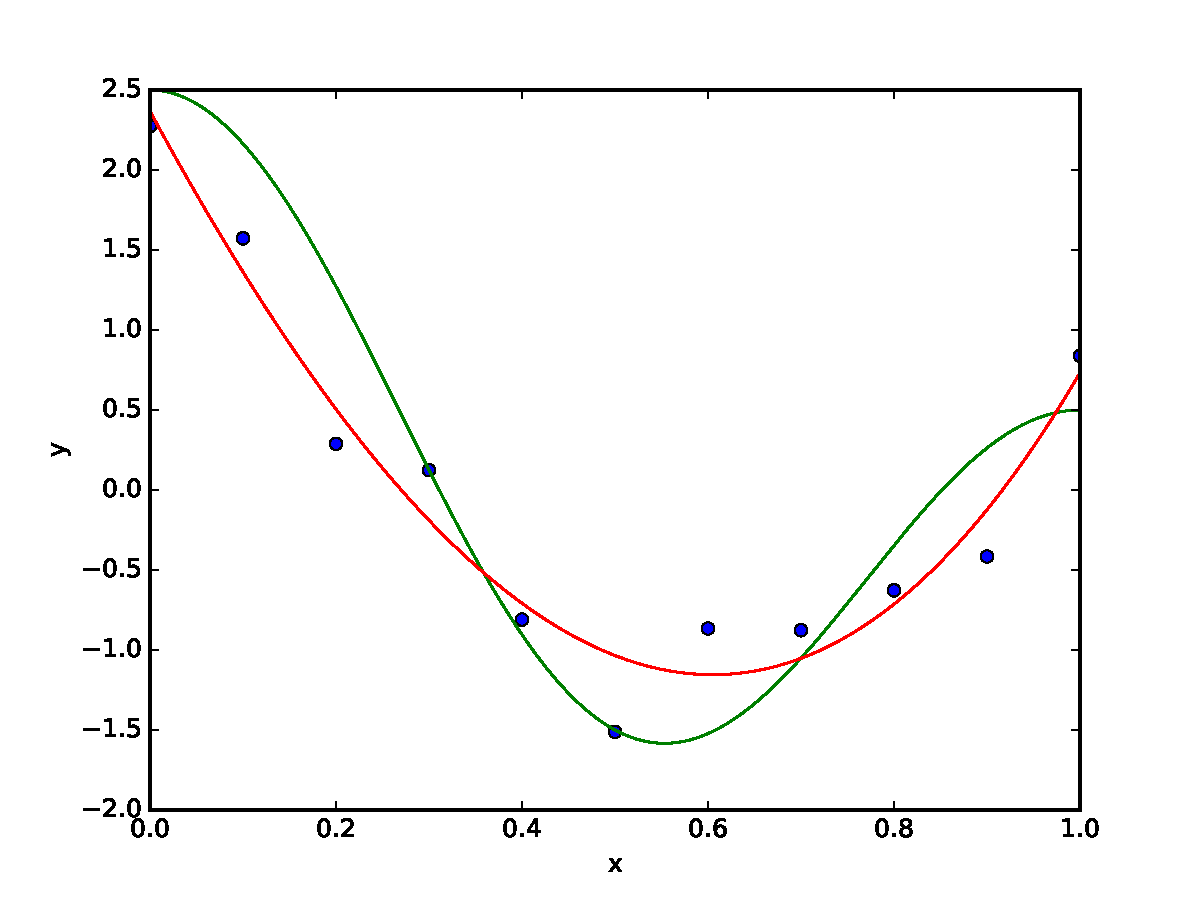
\includegraphics[width=\textwidth]{hw1_2-1_3.pdf}
		\caption{$M=3$}
	\end{subfigure}
	\begin{subfigure}[b]{0.24\textwidth}
		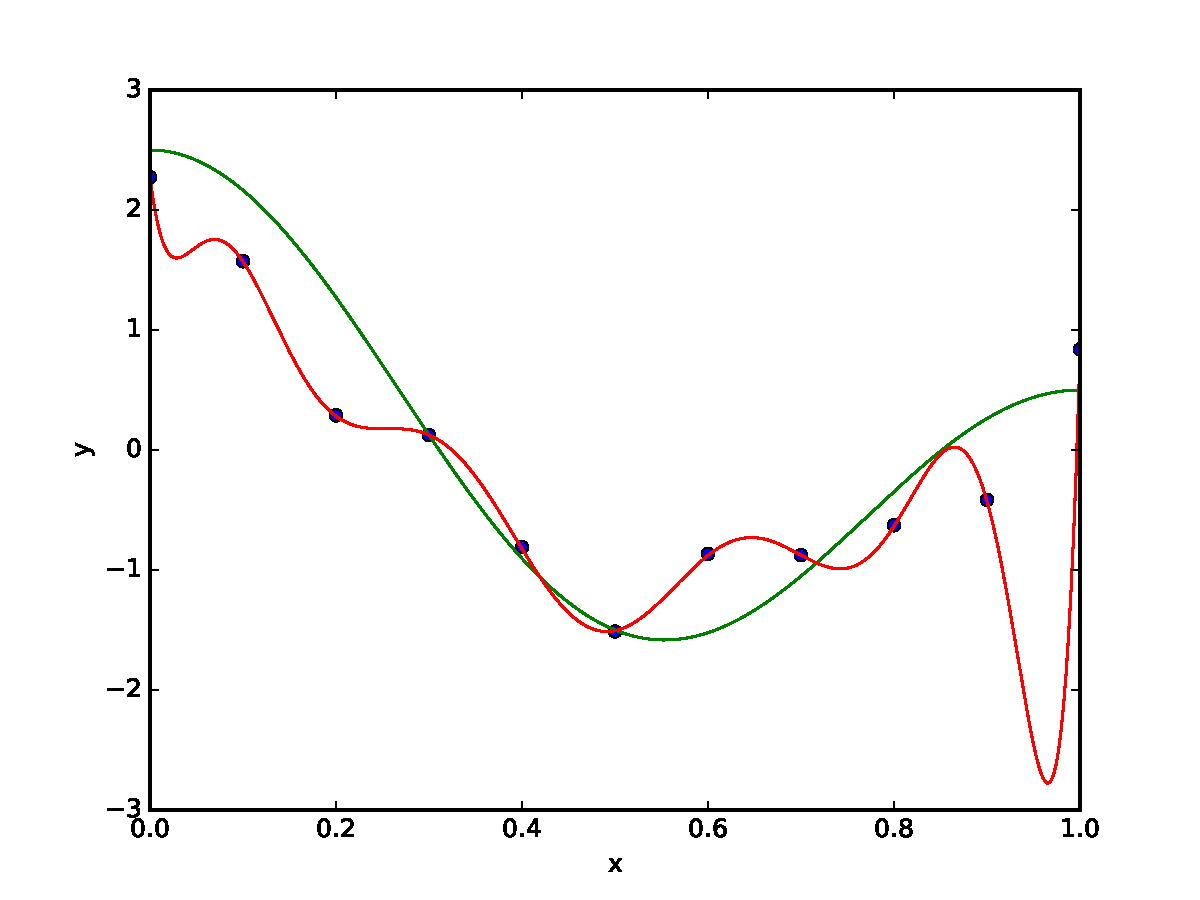
\includegraphics[width=\textwidth]{hw1_2-1_10.pdf}
		\caption{$M=10$}
	\end{subfigure}
	\caption{Polynomial fits to the cosine model, where the green line is the true model and the red line is the polynomial fit of degree $M$.}
\end{figure}

\subsection{SSE Loss} We define the SSE of the dataset and hypothesis as follows. The design matrix is given by:

$$\Phi \equiv \begin{pmatrix} \phi_0(x_1) & \phi_1(x_1) & \cdots & \phi_M(x_1) \\ \vdots & \vdots &  & \vdots \\ \phi_0(x_n) & \phi_1(x_n) & \cdots & \phi_M(x_n)\end{pmatrix}$$ 
where $\phi_i$ is the $i^{th}$ polynomial basis function, i.e. $\phi_i(x_j) = x_j^i$. Then the SSE for fixed weights $w = (w_0, w_1, \dots, w_M)$ is given by:
$$SSE(w) = \|\Phi w - y\|^2 = \sum_{i=1}^n (\Phi_{i\cdot}w - y)^2$$
in which $\Phi_{i\cdot}$ indicates the $i^{th}$ row of the design matrix. We can then easily derive the derivative of the squared error loss as in linear regression, which yields:

$$\nabla_w SSE(w) = 2 \Phi^T(\Phi w - y)$$

Verifying the gradient with the numerical finite difference approximations used in section 1.2, we find squared differences of order $10^{-13}$ tested at a number of weights with different dimensions ($w = (1,1), (5,3,4), (-5,5,-5,5), (1,10,1,10,-10,-1.1)$), increasing our confidence that the gradient is computing the correct update.

\subsection{Gradient-Based Methods for SSE Minimization} We now consider the choice of initialization, step size, and convergence thresholds for conducting batch GD and SGD. For all experiments, we use the best values of $\tau, \kappa$ found in the section 1.3; namely, we employ $\kappa = 10^{-5}$ and $\tau = 1$, and vary values of $w_0, \eta, \epsilon$. 

The results are shown in {\bf Figure 6}, in which we compare the squared distance of the solutions given by batch GD and SGD to the exact closed-form solution computed by maximum likelihood in section 2.1. We consider polynomial bases of order $M=1, 3, 5$ and initializations of the form (for $M = 3$) $w_0 = (1,1,1,1)$ and $w_0 = (5,5,-10,-10)$, with other orders analogously, to test whether large and asymmetric initial values can yield non-convergence. We vary $\eta = 10^{-1}, \dots, 10^{-3}$ and $\epsilon = 10^{-4}, \dots, 10^{-8}$, and display results for interesting cases; $w_0 = (5,-10)$ was almost identical to $w_0 = (1,1)$ and $w_0 = (1,1,1,1,1,1)$ was similar to $w_0 = (5,5,5,-10,-10,-10)$. We see that as in section 1.1, a sufficiently small step size $\eta$ is necessary for convergence for both batch GD and SGD, alongside a suitably small convergence threshold $\epsilon$ in nontrivial cases (i.e. $M \geq 3$). In gneeral, we found that $\epsilon \leq 10^{-8}$ was necessary for convergence. In more complex cases, however, SGD failed to converge to the exact solution even at these more precise convergence thresholds, unlike batch GD. This can result from generic problems faced by gradient-based methods in higher-dimensional spaces, namely getting stuck in local optima. For SGD, the issues are more acute because we are employing a noisy approximation to the true gradient by utilizing single samples, which can lead to the failure to converge even with small thresholds and step sizes.

\begin{figure}
	\centering
	\begin{subfigure}[b]{0.24\textwidth}
		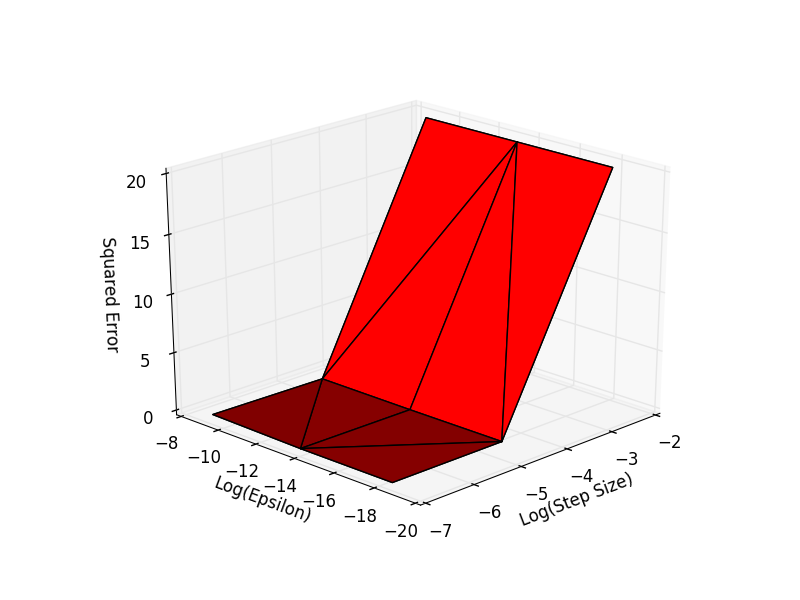
\includegraphics[width=\textwidth]{hw1_2-3_0.png}
		\caption{$w_0 = (1,1)$}
	\end{subfigure}
	\begin{subfigure}[b]{0.24\textwidth}
		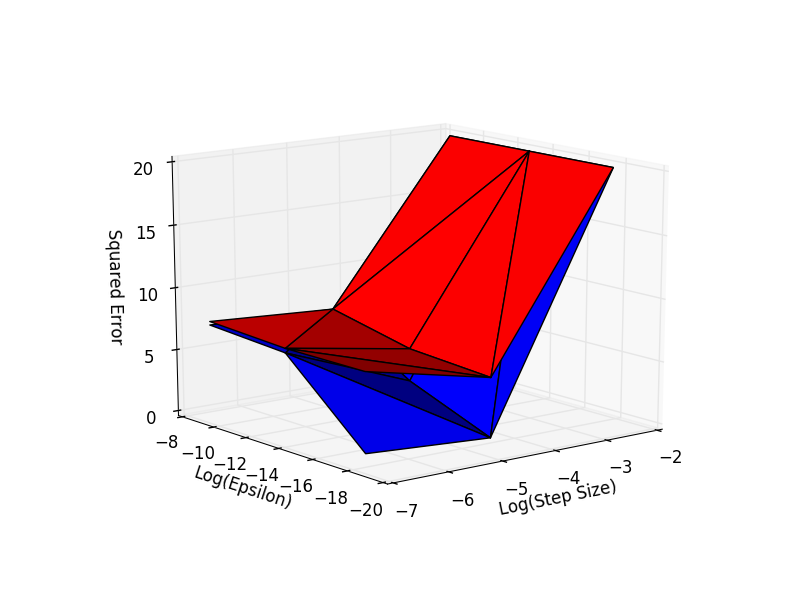
\includegraphics[width=\textwidth]{hw1_2-3_2.png}
		\caption{$w_0 = (1,1,1,1)$}
	\end{subfigure}
	\begin{subfigure}[b]{0.24\textwidth}
		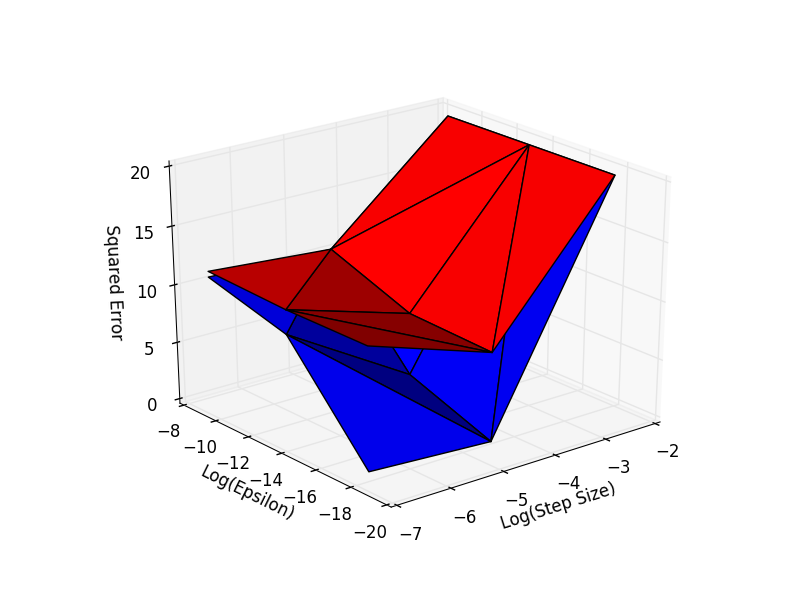
\includegraphics[width=\textwidth]{hw1_2-3_3.png}
		\caption{$w_0 = (5,5,-10,-10)$}
	\end{subfigure}
		\begin{subfigure}[b]{0.24\textwidth}
			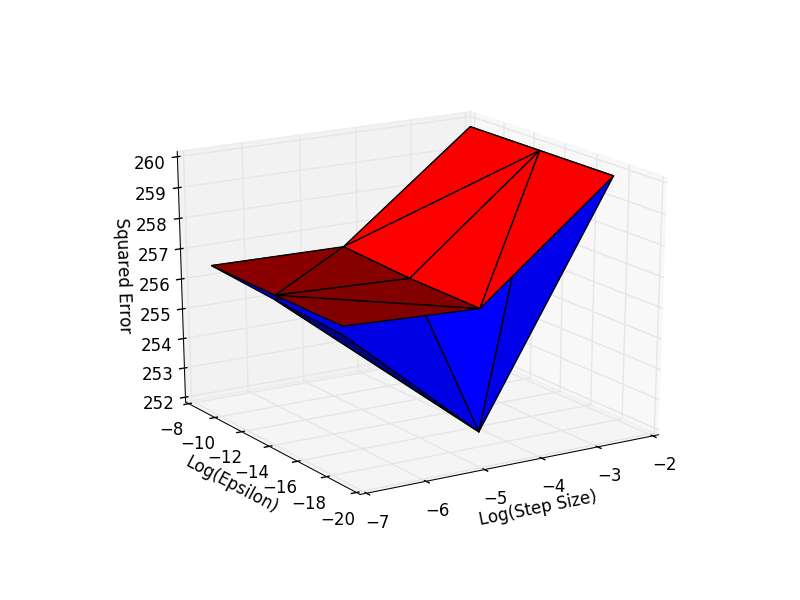
\includegraphics[width=\textwidth]{hw1_2-3_5.png}
			\caption{$w_0 = (5,5,5,-10,-10,-10)$}
		\end{subfigure}
	\caption{Squared error of batch GD and SGD solutions to exact SSE-minimizing solution for various initial weights, step sizes, and convergence thresholds.}
\end{figure}

\subsection{Cosine Basis} Finally, we assume that we know the function is given in a cosine basis, but do not know the order of the cosines used in generating the data nor the respective coefficients. We consider cosine functions of order 8:
$$\phi_1(x) = \cos(\pi x), \phi_2(x) = \cos(2\pi x), \dots, \phi_8(x) = \cos(8\pi x)$$
and use maximum likelihood as previously to estimate the weights for the functions. The MLE weights are approximately
$$\hat{w} = (0.77, 1.1, 0.1, 0.14, -0.05, 0.36, 0.01, 0.015)$$
and the plot of the true data-generating function and the MLE solution are given in {\bf Figure 7}. Interestingly, we see that the first two weights are in fact the largest by far in magnitude. However, as is common in maximum likelihood-based estimation, the weights overfit the data substantially, as seen in the red line in Figure 7. This is also implied by the MLE estimate $\hat{w}$; some of the magnitude of the first two weights (which should be $1, 1.5$ respectively) are ``siphoned off'' in a sense to the higher-order weights in order to fit the observed values more closely.

\begin{figure}
	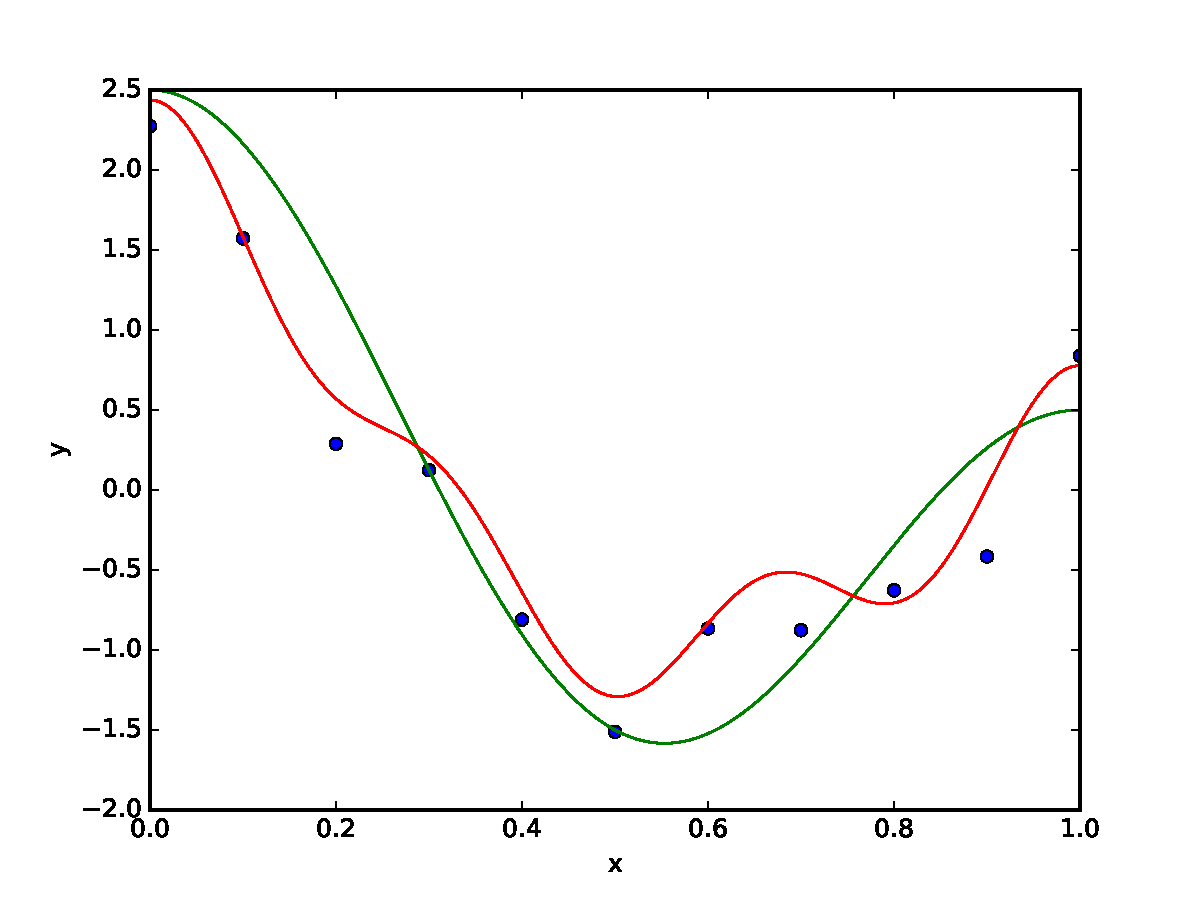
\includegraphics[width=0.25\textwidth]{hw1_2-4.pdf}
	\caption{The true data-generating function (green) compared to the MLE solution using an order-8 cosine basis (red).}
\end{figure}


\section{Ridge Regression}

\subsection{Polynomial Basis Example} One way to deal with the issue of overfitting faced in the cosine function example is to use a regularization method. A method for linear regression is ridge regression, which adds a quadratic weight decay term to the loss:
$$E(w) = \frac{1}{2}\|\Phi w - y\|^2 + \frac{\lambda}{2} w^Tw$$
which has a closed-form solution of:
$$w = (\Phi^T\Phi +\lambda I)^{-1} \Phi^T y$$
We investigate the capacity of ridge regression to combat overfitting issues by considering a polynomial basis of size $M = 3, 5, 8, 10$ (i.e. higher-order than the true function, so that overfitting is an issue) and vary the $\lambda = 0, 0.1, 0.5, 1, 10$ to see the impact on the resulting weights. {\bf Figure 8} illustrates our results.

\begin{figure}
	\centering
	\begin{subfigure}[b]{0.24\textwidth}
		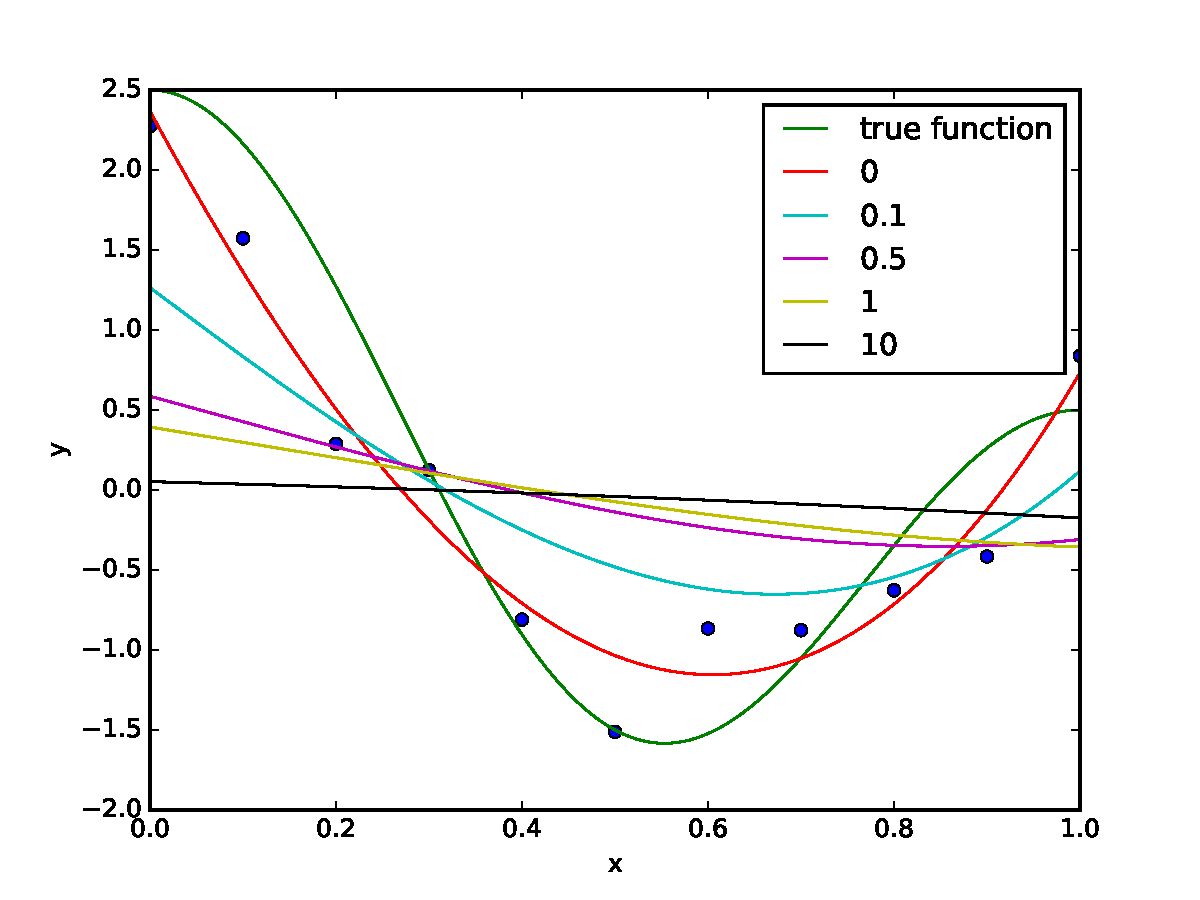
\includegraphics[width=\textwidth]{hw1_3-1_3.pdf}
		\caption{$M=3$}
	\end{subfigure}
	\begin{subfigure}[b]{0.24\textwidth}
		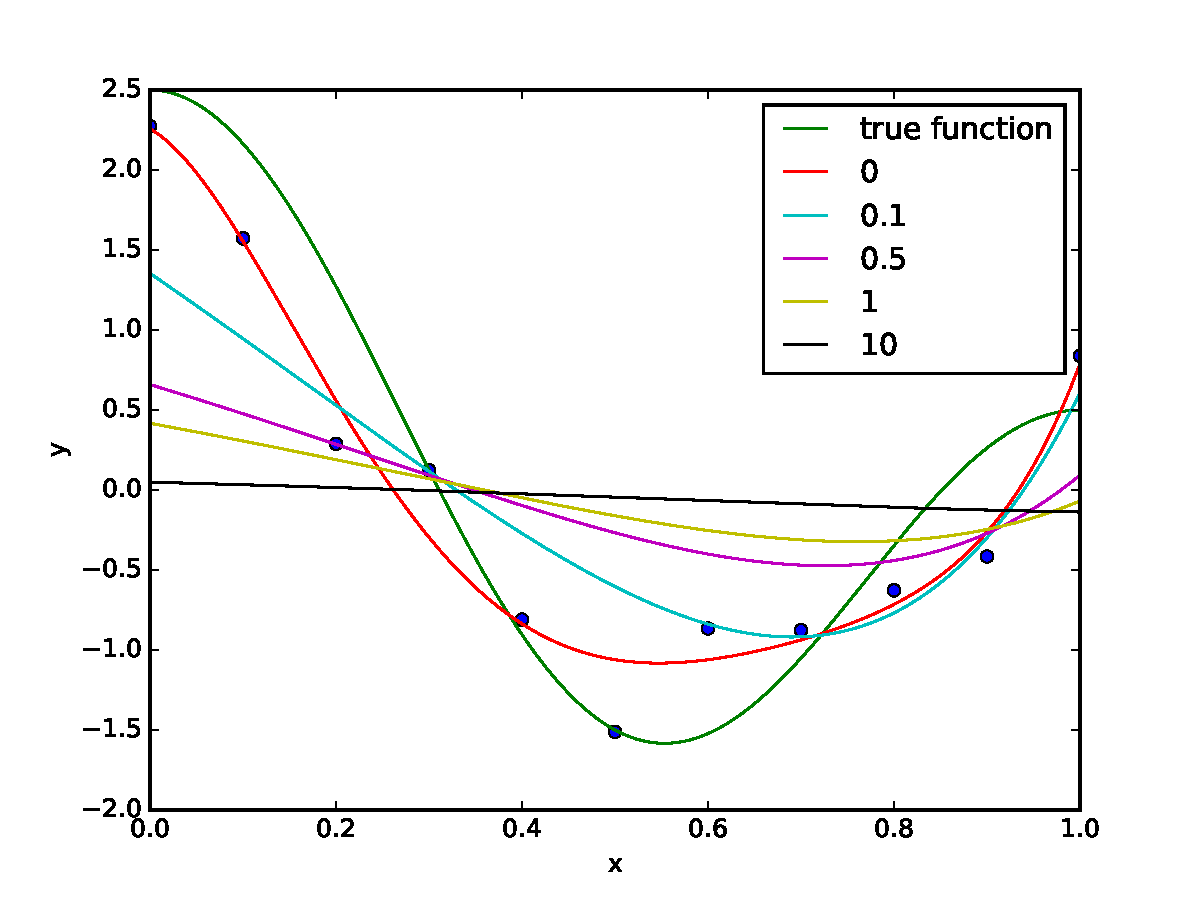
\includegraphics[width=\textwidth]{hw1_3-1_5.pdf}
		\caption{$M=5$}
	\end{subfigure}
	\begin{subfigure}[b]{0.24\textwidth}
		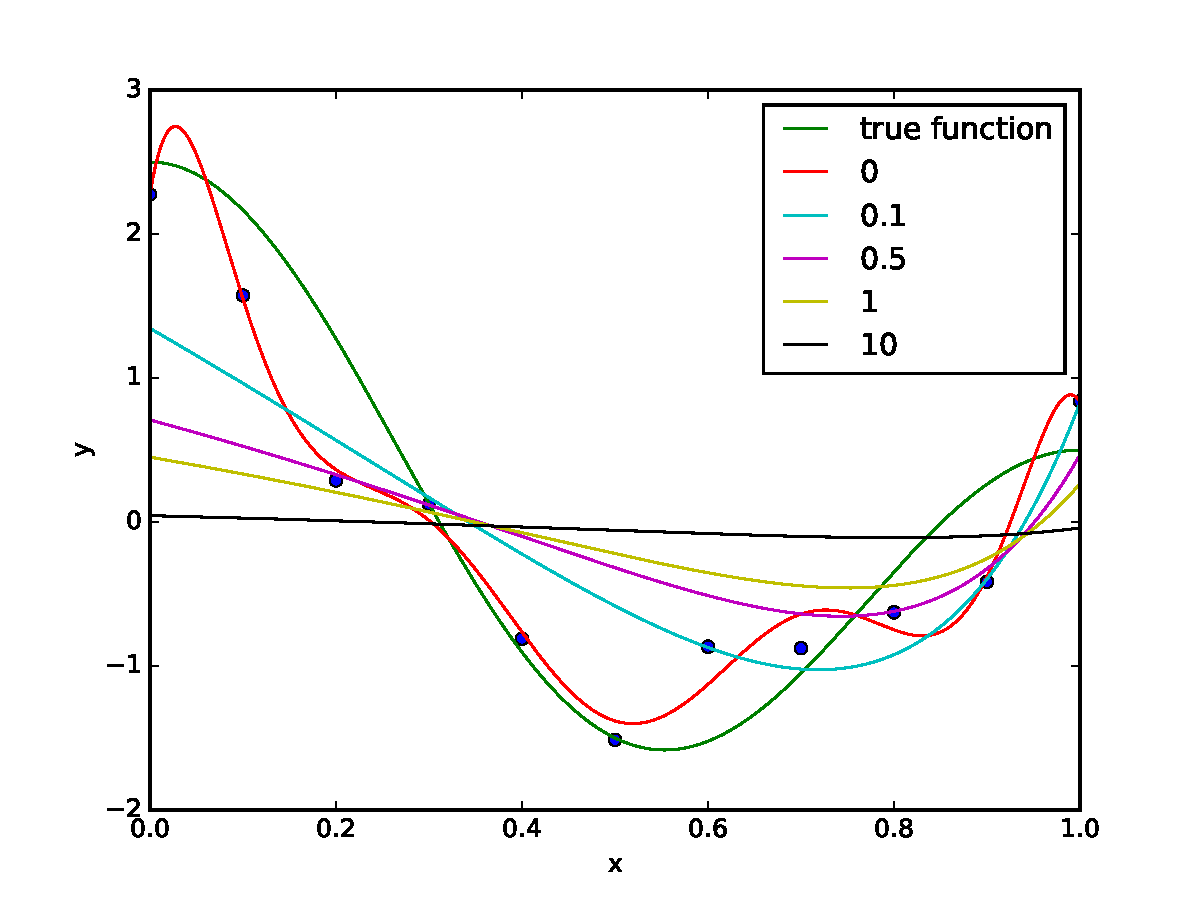
\includegraphics[width=\textwidth]{hw1_3-1_8.pdf}
		\caption{$M=8$}
	\end{subfigure}
	\begin{subfigure}[b]{0.24\textwidth}
		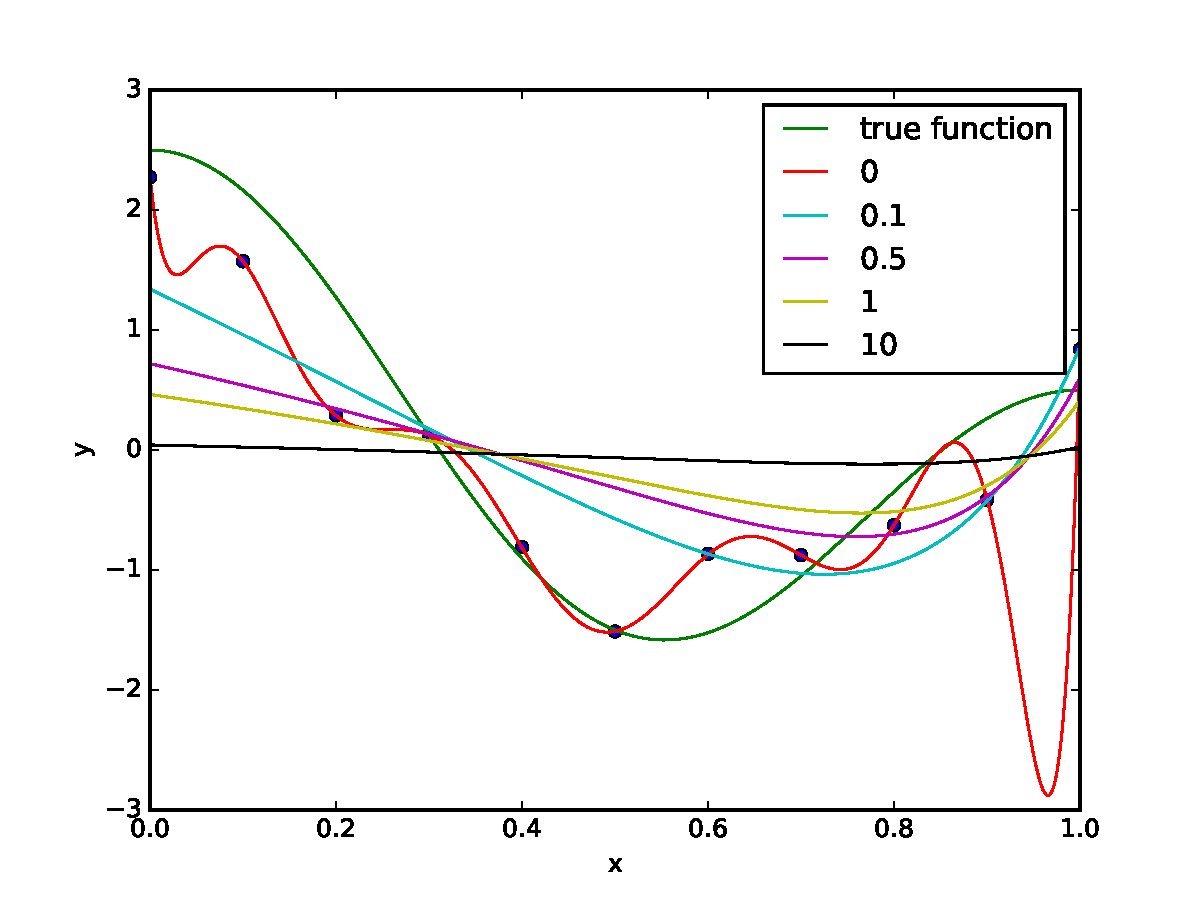
\includegraphics[width=\textwidth]{hw1_3-1_10.pdf}
		\caption{$M=10$}
	\end{subfigure}
	\caption{Ridge regression estimated weights for the cosine function data, using a cosine basis of order $M$.}
\end{figure}

We see that for higher-order polynomial bases, such as $M = 8, 10$, we overfit when $\lambda$ is small, i.e. $\lambda \leq 0.1$. For lower-order polynomial bases, such as $M = 3, 5$, no regularization seems to perform arguably better than high values of regularization, which implies that at $\lambda > 0.1$, the minimization of the error focuses too much on yielding weight decay rather than fitting the data properly. On the other hand, for $M = 8, 10$, one can claim that no $\lambda$ value yields a reasonable fit to the data. Low $\lambda$ values, as previously noted, yield high overfitting and low generalization properties, whereas high $\lambda$ values, while smoothing out the function, does not do so in the desired manner. Namely, we would like higher-order polynomial terms to have negligible weight and lower-order cosine terms to dictate the behavior of the fit. However, what we obtain is a consistently low weight parameter across orders, yielding a flat fit. Thus, ridge regression does not yield a satisfactory result on this example.

\subsection{Model Selection Using Validation Set} In the previous example, it was difficult to know {\em a priori} which values of $M, \lambda$ to choose to yield the best fit to the data. Even when we knew the data-generating function, it was unclear when we would err on the side of too low $M$ or too high $\lambda$. Thus, it is preferable to be able to select among various values of $M$ and $\lambda$ after actually fitting the data with these values. We can do so by testing our fit among many $M, \lambda$, trained on the training set, on a separate validation set.

In this example, we return to the polynomial basis and consider the same ridge regression setup using this basis. We use three sets of data: training set A, training set B, and validation set. We explore how the choice of which sets to use as the training and test sets affects the selected model we obtain at the end of the process, using either A as test and B as train, or vice-versa. We investigate $M = 1, 3, 5, 7$ with $\lambda = 0, 0.1, 0.5, 1, 5, 10$ as the possible hyperparameter values.

{\bf Figure 9(a,c)} demonstrates the results, where the selected model (i.e. minimum squared error on validation set) is shown as a bold line and the rest of the fits are dotted. The points shown in the plots are the test set (i.e. B if trained on A). {\bf Figure 9(b,d)} then report on the squared error of the various fits on the validation set. We found that $M = 3$ is selected via model selection in both cases. On the other hand, $\lambda = 0$ (i.e. no regularization) works best when set A is used as the training set, whereas $\lambda = 0.5$ is selected when set B is used for training. This reveals that due to the outlier value in set B, more regularization (nonzero $\lambda$) is necessary to prevent overfitting to this outlier value, compared to the very regular (and linear) data in the validation set. This is visible in Figure 9(c), where the non-bold fits (i.e. not chosen during model selection) generally reveal severe overfitting to the outlier point in set B.

\begin{figure}
	\centering
	\begin{subfigure}[b]{0.24\textwidth}
		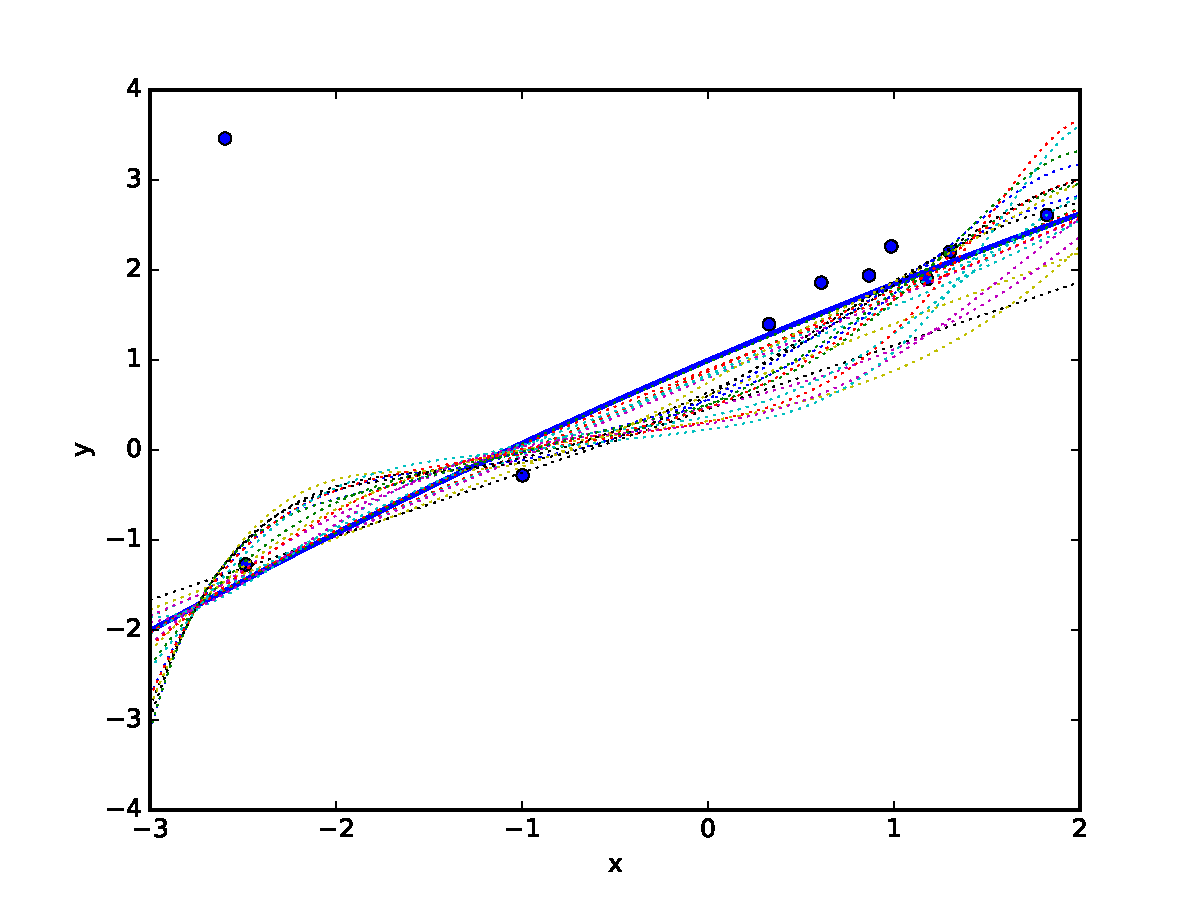
\includegraphics[width=\textwidth]{hw1_3-2_A.pdf}
		\caption{Training set A, test set B}
	\end{subfigure}
	\begin{subfigure}[b]{0.24\textwidth}
		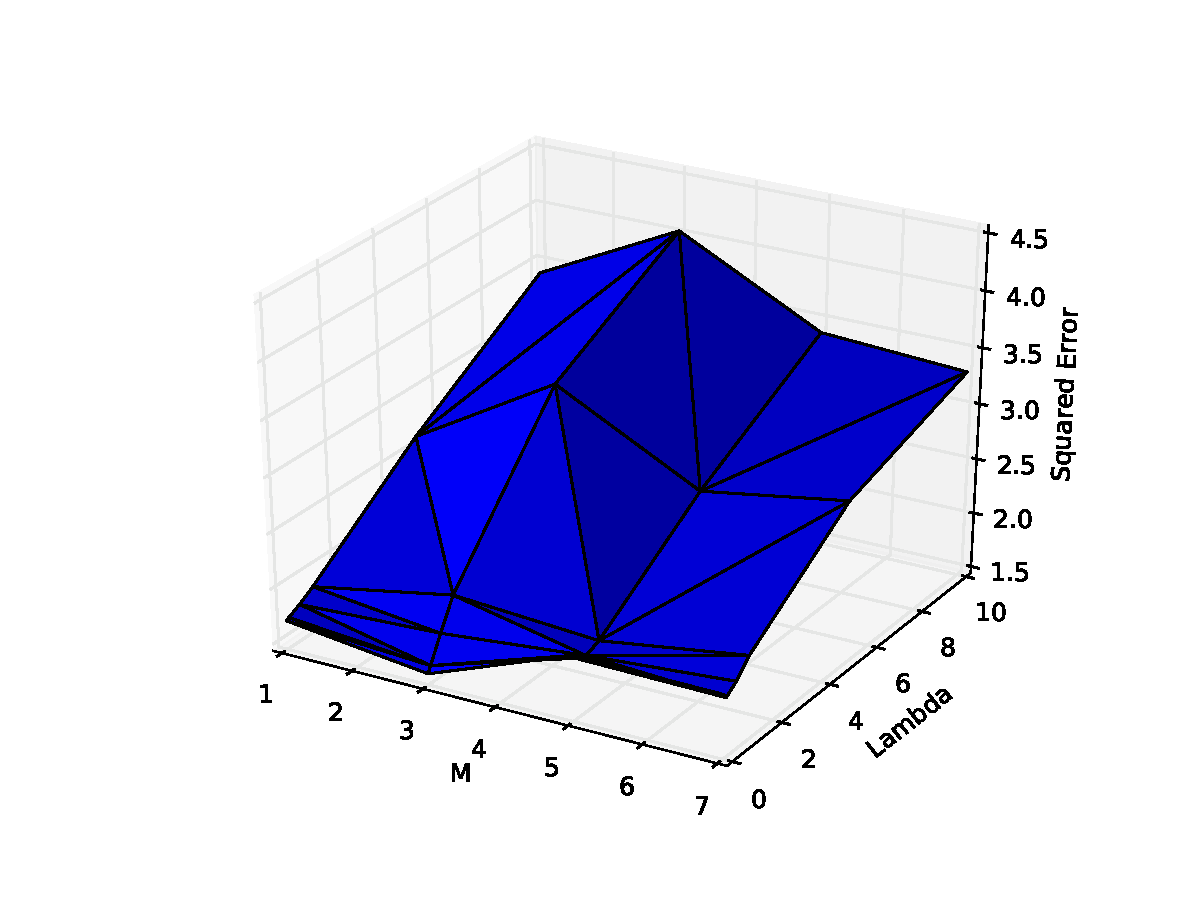
\includegraphics[width=\textwidth]{hw1_3-2_A_err.pdf}
		\caption{Validation error (train A)}
	\end{subfigure}
	\begin{subfigure}[b]{0.24\textwidth}
		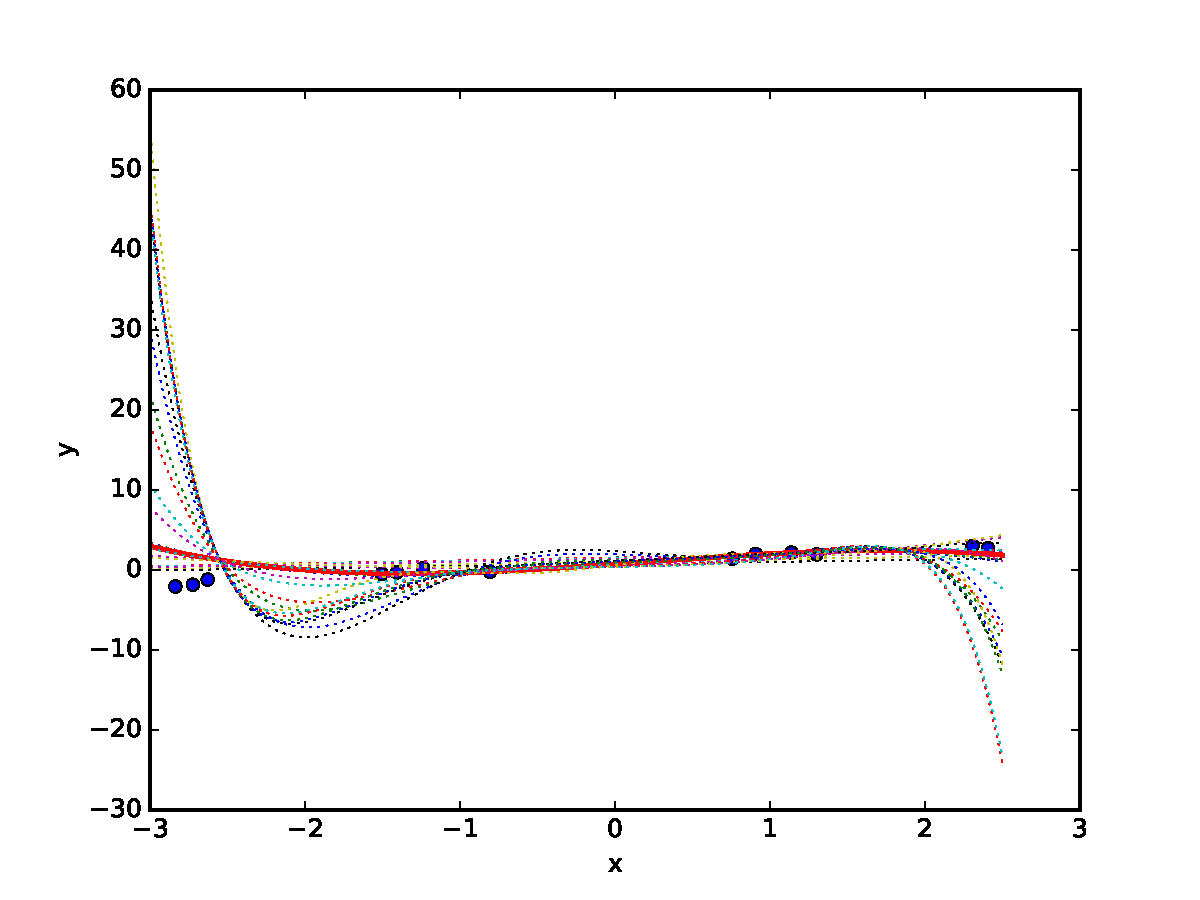
\includegraphics[width=\textwidth]{hw1_3-2_B.pdf}
		\caption{Training set B, test set A}
	\end{subfigure}
	\begin{subfigure}[b]{0.24\textwidth}
		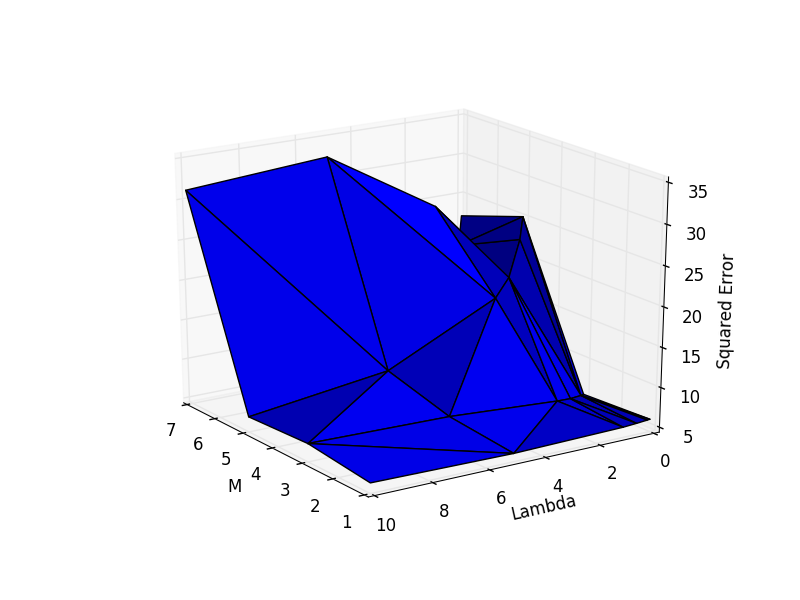
\includegraphics[width=\textwidth]{hw1_3-2_B_err.png}
		\caption{Validation error (train B)}
	\end{subfigure}
	\caption{Ridge regression estimated weights using a polynomial basis of order $M$ and weight decay penalty of $\lambda$.}
\end{figure}

\section{Sparsity and LASSO}

The problem with ridge regression in the previous examples, whether with the polynomial or cosine bases, was that we did not desire for the weights of all order terms to shrink, but rather for some terms to have zero weights and more important terms to have full weights. Namely, we wanted sparse weights, rather than uniformly smaller weights. To achieve this goal, we employ LASSO regression, rather than ridge regression. Instead of the $L^2$ norm of the weights, LASSO penalizes the absolute value of the weights:
$$E(w) = \frac{1}{2}\|\Phi w-y\|_2^2 + \frac{\lambda}{2}\|w\|_1$$
where $\|\cdot\|_1$ is the $L^1$ or absolute value norm. To explore how LASSO yields sparse weights for regression, we use the model:
$$y = w^T\phi(x)  + \epsilon$$
where again $\epsilon$ is random noise and $\phi(x) = = (x,\sin(0.4\pi x \cdot1),\sin(0.4\pi x \cdot 2), . . . ,\sin(0.4\pi x \cdot 12))$ is the true basis. The true data-generating weights are: 
$$w = (0,0, 5.6463, 0.7786,0, 0.8109,2.6827, 0,0,0,0,0,0 )$$
which is very sparse (only 4 out of 13 weights are nonzero). We again use various values of $\lambda$ for regularization in both ridge and LASSO regression, showing only the best value of $\lambda$ as selected through model selection procedures on the validation set. Due to the small size of the training set, we use batch proximal gradient descent to optimize the LASSO loss, using $\epsilon = 10^{-15}$ and step size equal to $\lambda$ during all experiments (the max number of iterations is set to $10^{4}$ so that the algorithm terminates). Finally, we initialize all values at 1 to start any gradient descent process. Note that the MLE is ill-defined for this problem, as there are fewer training points than there are covariates (i.e. $n = 5$ but $p = 13$) so there are multiple solutions. We opt for the most principled method, namely the ``least squares solution'', which computes:
$$\hat{w} = \Phi^T(\Phi \Phi^T)^{-1} y$$
We can achieve arbitrarily bad MLE fits by using a gradient descent procedure at large initial values (i.e. setting every initial weight to, say, $10^2$) but we opt not to set up a strawman example by pursuing the most reasonable course, which is to prefer the solution with the smallest $L_2$ norm weights, for parsimony and generalizability.

The main result is illustrated by {\bf Figure 10}, which plots the estimated functions using MLE, ridge, and LASSO regressions against the true function. We plot only the estimated fit for the weights that yield the lowest squared error on the validation set. We find that all of the methods do similarly well in terms of performance on the test set. In fact, the LASSO fit has the highest SSE on the test data, and the MLE has the lowest (estimated using least norm). This is most likely due to the similarity between the training, validation, and test sets in this example, so that overfitting does not occur unless we initialize the weights at some unreasonably high value. For sparsity and generalizability, it is reasonable to initialize the weights at low values as done in this example, which yields reasonable fits even without regularization.

However, {\bf Figure 11} reveals that despite the performance of the MLE and ridge regression estimates on the test data, they fail to capture the sparsity in the weights that is exhibited by the true weights. There are significantly nonzero values across almost all the weights, which is not characteristic of the true solution. On the other hand, the LASSO solution, while failing to perform better in terms of predictive power on the test set, does manage to capture this sparsity extremely well, yielding estimates that are very similar to the true weights. This is also revealed by Figure 10(c), which shows that the LASSO solution is very close in $L_2$ distance to the true weights, compared to the MLE or ridge solutions.

\begin{figure}
	\centering
	\begin{subfigure}[b]{0.25\textwidth}
		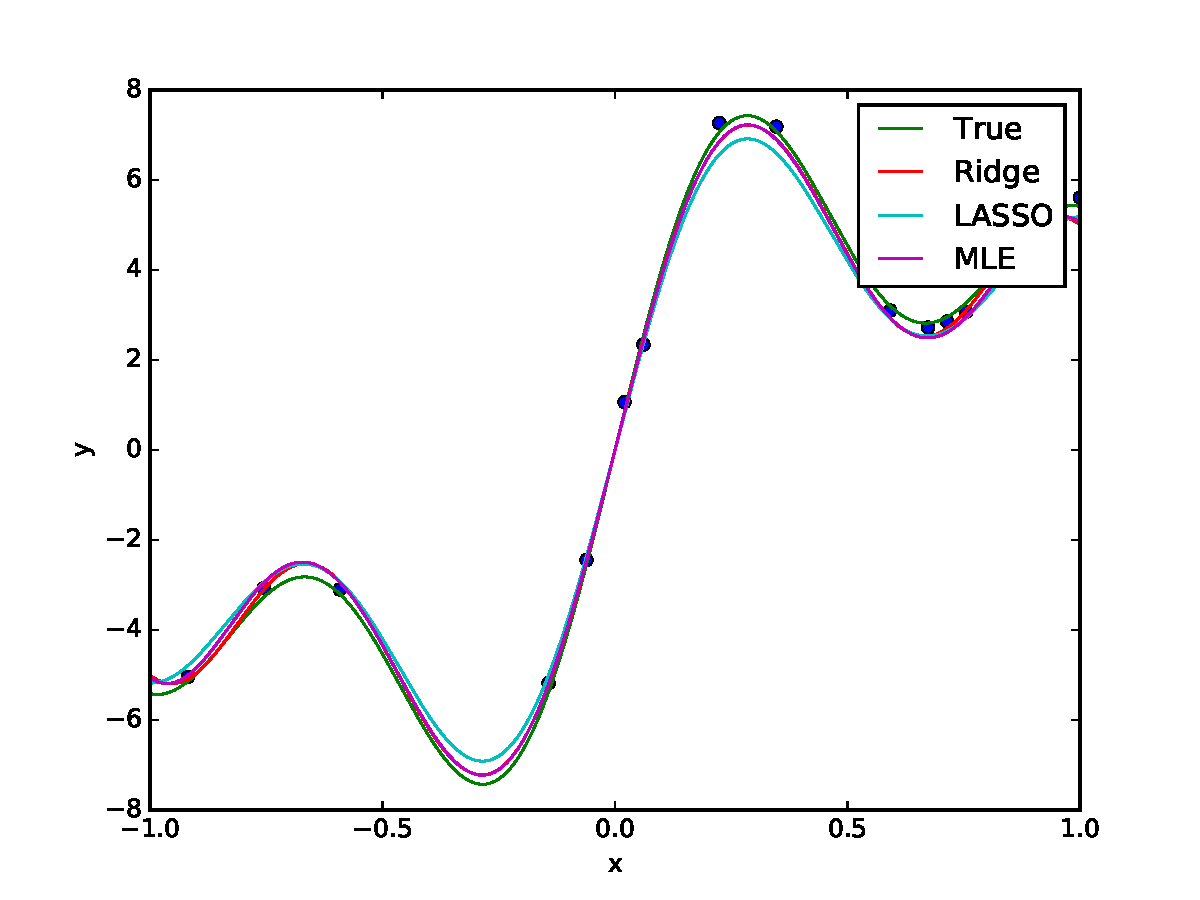
\includegraphics[width=\textwidth]{hw1_4-1.pdf}
		\caption{Fit on test}
	\end{subfigure}
	\begin{subfigure}[b]{0.25\textwidth}
		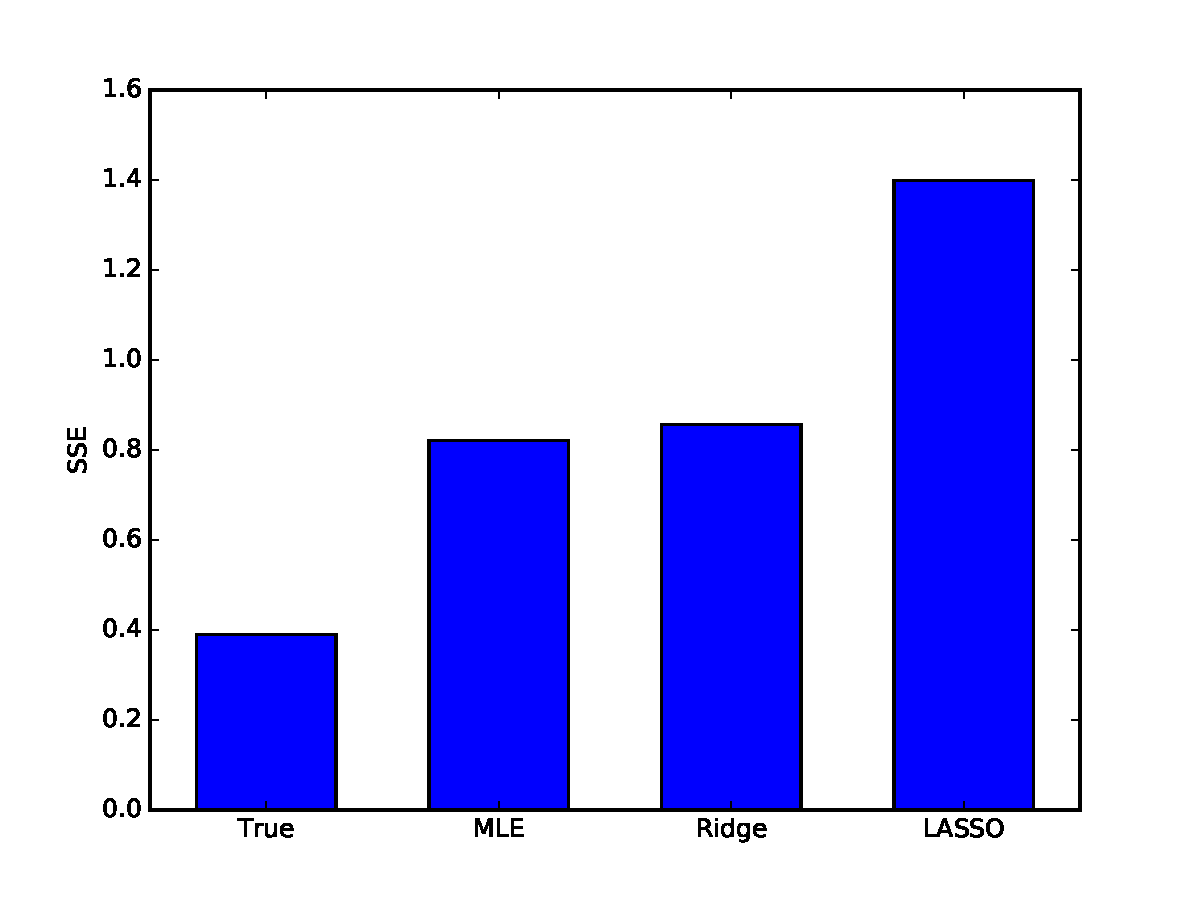
\includegraphics[width=\textwidth]{hw1_4-1_2.pdf}
		\caption{SSE on test}
	\end{subfigure}
	\begin{subfigure}[b]{0.25\textwidth}
		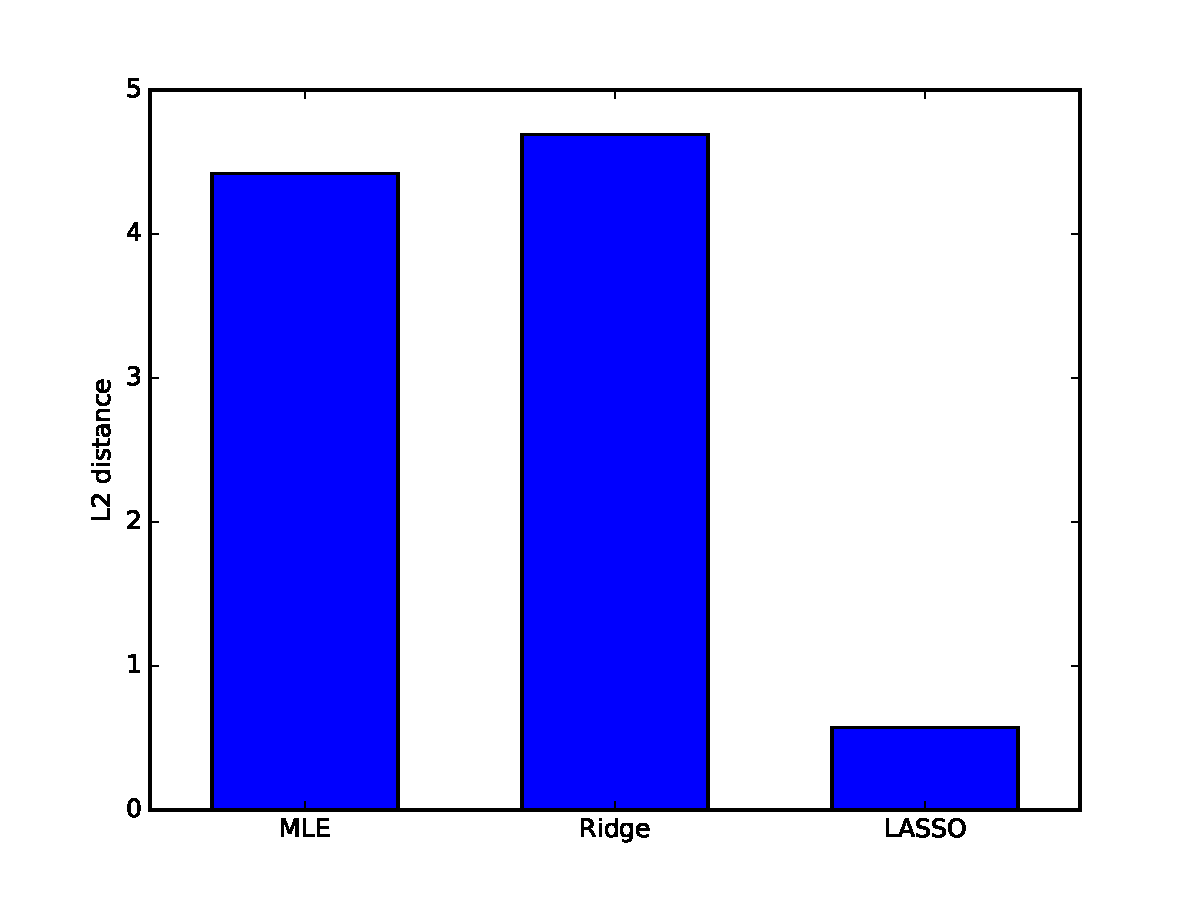
\includegraphics[width=\textwidth]{hw1_4-1_3.pdf}
		\caption{$L_2$ distance to true}
	\end{subfigure}
	\caption{Estimated fits to the data using MLE, ridge regression, and LASSO and the associated SSE on the test data and $L_2$ distance to the true weights.}
\end{figure}

\begin{figure}
	\centering
	\begin{subfigure}[b]{0.24\textwidth}
		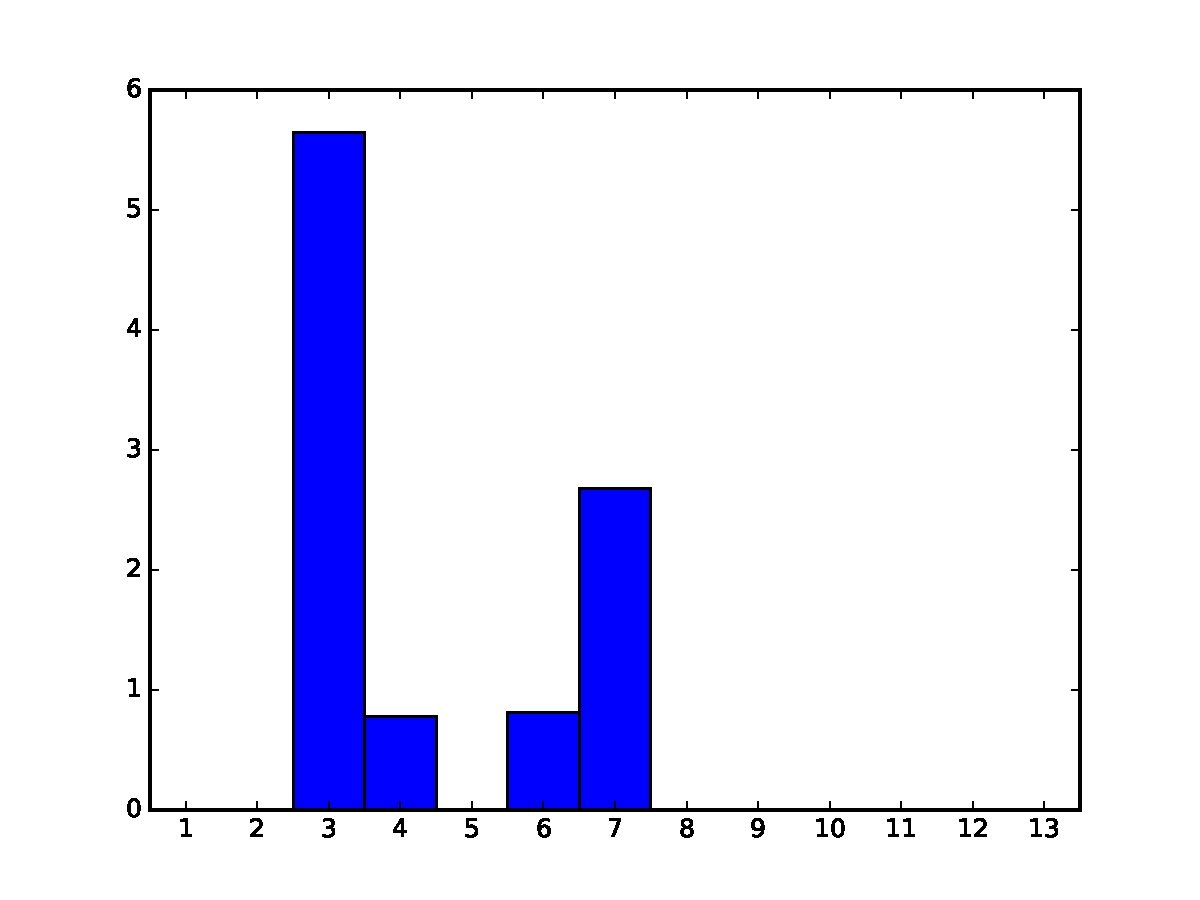
\includegraphics[width=\textwidth]{hw1_4-2_1.pdf}
		\caption{True weights}
	\end{subfigure}
	\begin{subfigure}[b]{0.24\textwidth}
		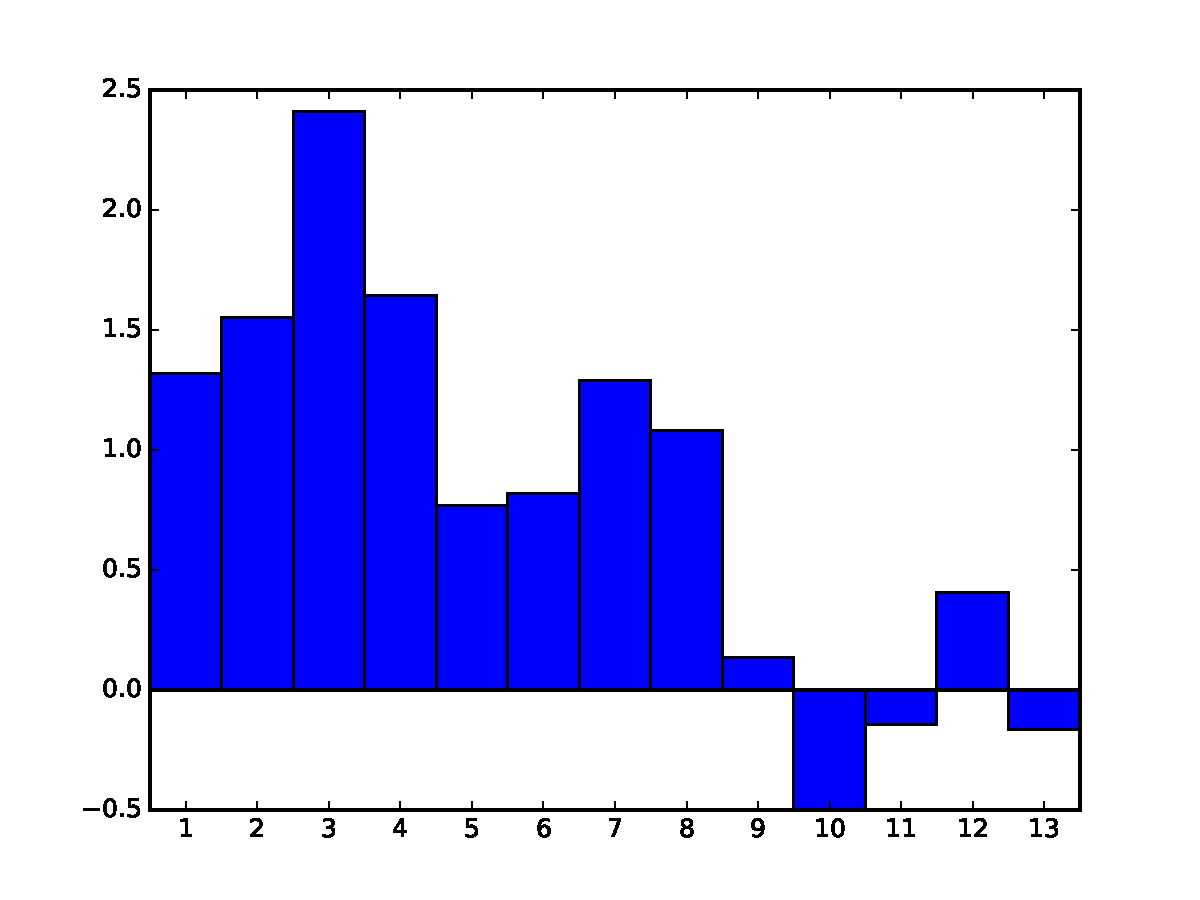
\includegraphics[width=\textwidth]{hw1_4-2_2.pdf}
		\caption{MLE}
	\end{subfigure}
	\begin{subfigure}[b]{0.24\textwidth}
		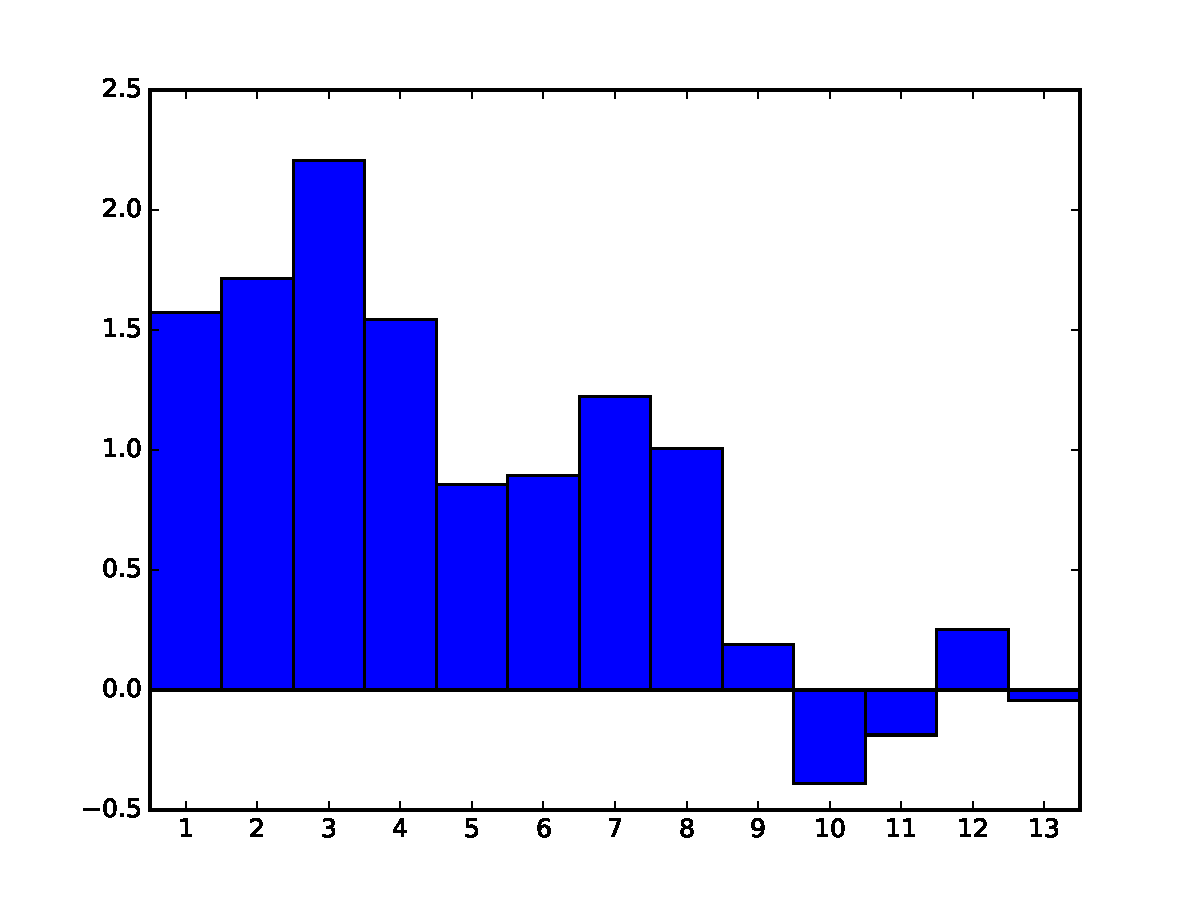
\includegraphics[width=\textwidth]{hw1_4-2_3.pdf}
		\caption{Ridge}
	\end{subfigure}
	\begin{subfigure}[b]{0.24\textwidth}
		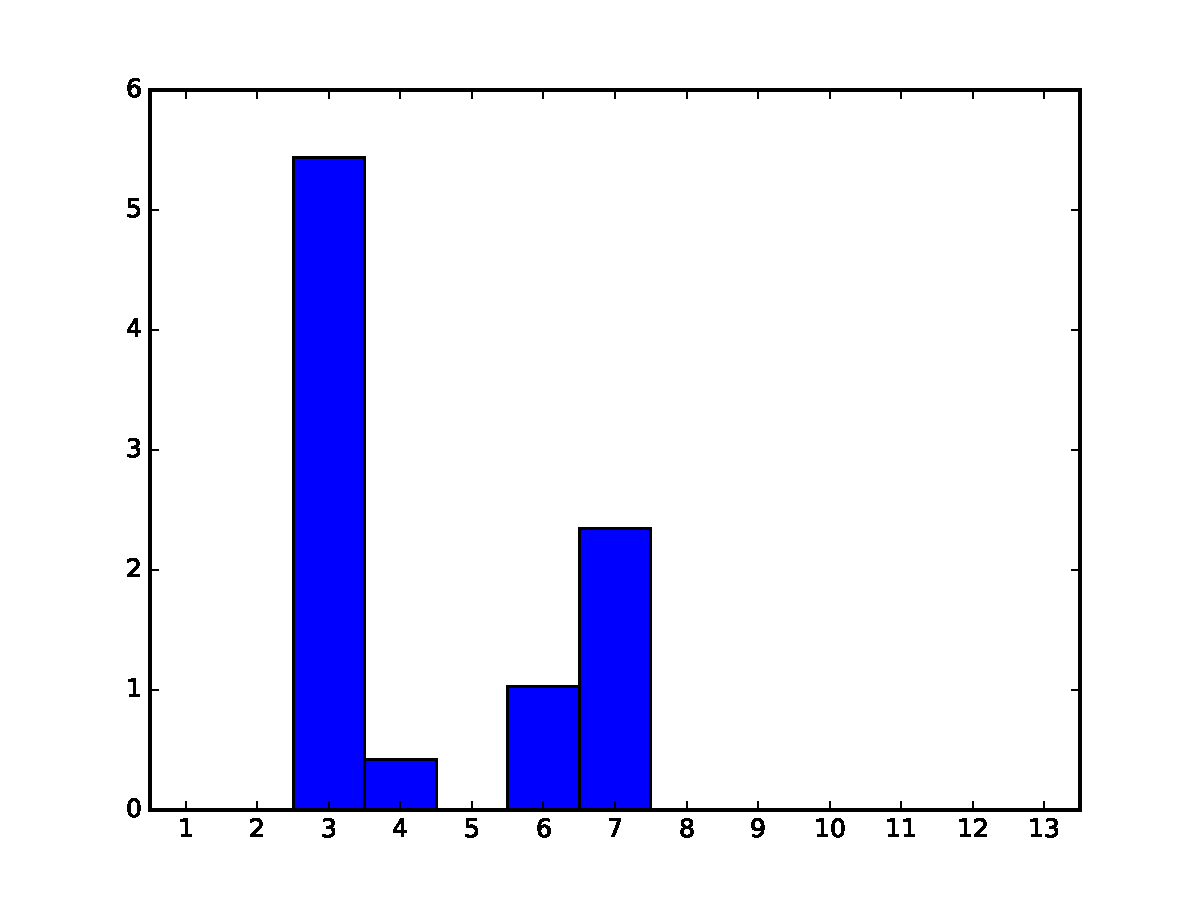
\includegraphics[width=\textwidth]{hw1_4-2_4.pdf}
		\caption{LASSO}
	\end{subfigure}
	\caption{Estimated weights with lowest validation error, for MLE, ridge, and LASSO regressions, compared to true weights.}
\end{figure}

\end{document}


